% node start (ID_806462407)
% TEXT = Marker locator% node end (ID_806462407)
% node start (ID_327218372)
% TEXT = preamble
\documentclass{article} 
\usepackage{textcomp} 
\usepackage{amsmath} 
\usepackage[font=it,labelfont=bf]{caption} 
\usepackage{graphicx} 
\usepackage{subcaption} 
\usepackage{biblatex} 
\usepackage{tikz} 
\usepackage{todonotes} 
\addbibresource{papers.bib} 
\usepackage[danish]{babel} 
\usepackage[colorlinks, linkcolor=blue, urlcolor=blue, citecolor=blue]{hyperref} 
 
\title{Robust detection of n-fold edges using convolution with a complex kernel} 
\author{Henrik Skov Midtiby} 
 
\begin{document} 
\maketitle 
% node end (ID_327218372)
% node start (ID_1746758294)
% TEXT = abstract
\begin{abstract} 
In some cases it is required to track a certain point / marker on an object in an image / a sequence of images. 
This paper suggest to use a marker (an n-fold edge) constructed by repeating a 
pattern of white and black regions $n$ times. 
The center of the marker can then be located by a convolution with a kernel containing complex numbers. 
\end{abstract} 
% node end (ID_1746758294)
% node start (ID_841329411)
% TEXT = Introduction
\section{Introduction} 
% node end (ID_841329411)
% node start (ID_508314549)
% TEXT = Requirement% node end (ID_508314549)
% node start (ID_356287990)
% TEXT = Locate certain objects in images
An often occuring task in computer vision is to locate a certain object or position in an image. 
It can either be a generic object, or an object (a marker) that the user have placed actively in the field of view. 
Robust detection of one or more markers can give precise pose estimates which are required for applications like Augmented Reality. 
 
% node end (ID_356287990)
% node start (ID_259481509)
% TEXT = Others approach
Many types of markers have been suggested, and they can be divided into two types of markers. 
The first type of markers are intended for estimating the pose of the object on which the marker is placed. 
This requires at least four points to be identifiable in the marker, which often consists of a square or rectangular 
array of black and white pixels. 
QR Codes and ARuCo markers are both of this type. 
The second type of markers identifies specific points in images. 
These markers resemble eg. chess board corners and log spirals. 
 
% node end (ID_259481509)
% node start (ID_709786542)
% TEXT = QR codes
QR Codes are a 2D bar code, that can contain a significant amount of information. 
The largest QR codes contain almost 3000 bytes of information. 
QR Codes was developed by DENSO WAVE. 
The minimum resolution for reading a QR code containing four bytes of information using the \url{https://zxing.org/w/decode.jspx} QR code decoder around 50 x 50 pixels (personal experiments). 
% Scaling down a QR code with the text "test" until it got so small / blurred that it was impossible to read the code. 
% node end (ID_709786542)
% node start (ID_362522283)
% TEXT = ARuCO
ARuCo markers consists of a black border with a $n \times n$ pattern of black and white pixels inside the border \cite{Garrido-Jurado2014}. 
The smallest ARuCo marker consists of $4 \times 4$ pixel within an two pixel wide border made of black and white pixels. 
To detect this marker a resolution of at least 18 pixels is likely needed. 
% node end (ID_362522283)
% node start (ID_1150681358)
% TEXT = Chess board corners
Chess board corners are regularly used for camera calibration. 
The corners can be detected using different techniques, eg. the Harris corner detector \cite{Harris1988}. 
% node end (ID_1150681358)
% node start (ID_1461471088)
% TEXT = Log spirals
A marker formed as a logarithmic spiral was suggested in \cite{Karlsson2011}. 
A visual comparison of the mentioned marker types are given 
in figure \ref{figExampleMarkerTypes}. 
 
% node end (ID_1461471088)
% node start (ID_791196354)
% TEXT = figExampleMarkerTypes
\begin{figure} 
\begin{tikzpicture} 
\draw (0, 0) node[right, align=left]{QR Code \\ $48 \times 48$}; 
\draw (5, 0) node{
\includegraphics[width=2cm]{pic/markertypes/qr_code_230x230.png}}; 
\draw (8, 0) node{
\includegraphics[width=2cm]{pic/markertypes/qr_code_48x48.png}}; 
\draw (0, -2) node[right, align=left]{ARuCo \\ $25 \times 25$}; 
\draw (5, -2) node{
\includegraphics[width=2cm]{pic/markertypes/aruco_250x250.png}}; 
\draw (8, -2) node{
\includegraphics[width=2cm]{pic/markertypes/aruco_25x25.png}}; 
\draw (0, -4) node[right, align=left]{Logspiral \\ $21 \times 21$}; 
\draw (5, -4) node{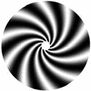
\includegraphics[width=2cm]{pic/markertypes/logspiral_91x91.png}}; 
\draw (8, -4) node{
\includegraphics[width=2cm]{pic/markertypes/logspiral_21x21.png}}; 
\end{tikzpicture} 
\caption{Examples of different marker types and images with 
a minimal resolution in which the marker can be detected (and verified).} 
\label{figExampleMarkerTypes} 
\end{figure} 
% node end (ID_791196354)
% node start (ID_1668285930)
% TEXT = Goals and means
This paper suggests a new marker design with the following properties 
1) robust detection of the marker, 
2) the algorithm requires no segmentation of the input image prior to marker detection and 
3) the algorithm can locate low resolution markers. 
This is achieved by analysing the neighbourhood around each pixel in the image, like in the FAST corner dector \url{http://www.edwardrosten.com/work/fast.html}. 
The analysis is done by convolution of the image with a kernel containing complex.values. 
This approach limits the algorithm to only locate markers with a certain fingerprint. 
 
% node end (ID_1668285930)
% node start (ID_1518320303)
% TEXT = Define a marker that is robust to detect.% node end (ID_1518320303)
% node start (ID_674566423)
% TEXT = Require no segmentation for detection.% node end (ID_674566423)
% node start (ID_1039386918)
% TEXT = A marker that can be found with limited resolution% node end (ID_1039386918)
% node start (ID_1872198652)
% TEXT = Means% node end (ID_1872198652)
% node start (ID_344837613)
% TEXT = Fourier transformation around points in the image% node end (ID_344837613)
% node start (ID_621814960)
% TEXT = Concerns% node end (ID_621814960)
% node start (ID_949497313)
% TEXT = Can only detect certain markers% node end (ID_949497313)
% node start (ID_59842385)
% TEXT = No information stored in markers% node end (ID_59842385)
% node start (ID_1583702410)
% TEXT = Structure of this paper% node end (ID_1583702410)
% node start (ID_678276898)
% TEXT = Materials and methods
\section{Materials and methods} 
% node end (ID_678276898)
% node start (ID_357477363)
% TEXT = Convolution for detection of markers with fixed rotation
\subsection{Template matching} 
% node end (ID_357477363)
% node start (ID_525900738)
% TEXT = Template matching
It is possible to use template matching to locate objects with a fixed orientation in an image. 
\url{https://docs.opencv.org/trunk/d4/dc6/tutorial_py_template_matching.html} 
% node end (ID_525900738)
% node start (ID_1711581391)
% TEXT = Fourier transform
\subsection{Fourier transform} 
% node end (ID_1711581391)
% node start (ID_1907073549)
% TEXT = Discrete fourier transform
Given $N$ observations ($x_0$, $x_1$, \ldots), the $k$th term in 
the discrete Fourier transform is given by the equation: 
\[ 
X_{k}=\sum _{n=0}^{N-1} x_{n} \cdot e^{-i2\pi kn/N} 
\] 
% node end (ID_1907073549)
% node start (ID_1923185394)
% TEXT = Notice the pattern
Notice that the Discrete Fourier transform is a weighted sum over a set of observations, that is a convolution. 
In the standard situation the set of observations is sampled along a linear dimension. 
% node end (ID_1923185394)
% node start (ID_396153378)
% TEXT = Apply the pattern to a 2D input
Instead of sampling along a linear dimension, the sampling will be done over a 2D area, the kernel window. 
This is similar to a 2 D convolution, which is defined as follows: 
\[ 
f[x, y] \textasteriskcentered  g[x, y] = \sum_{k = -w}^{w} \sum_{l = -w}^{w} f[k, l] \cdot g(x - k, y - l) 
\] 
The task is now to design a pattern to add to the object that should be tracked 
and which is possible to detect with the convolution based approach described above. 
% node end (ID_396153378)
% node start (ID_1411063844)
% TEXT = Square wave
\subsection{Square wave} 
% node end (ID_1411063844)
% node start (ID_1002027442)
% TEXT = Square wave sine expansion
A square wave $x(t)$ with amplitude $1$ and frequency $f$ can be represented with the Fourier series 
\[ 
x(t)=\frac{4}{\pi} \left(\sin(2\pi ft)+\frac{1}{3} \sin(6 \pi f t) + \frac{1}{5} \sin(10 \pi f t) + \ldots \right) 
\] 
Given the function $x(t)$, the Fourier transform can be used to determine the elements 
of the Fourier series. 
% node end (ID_1002027442)
% node start (ID_973884286)
% TEXT = Square wave expansion in complex exponentials% node end (ID_973884286)
% node start (ID_72772172)
% TEXT = Shifts in the pattern can be detected by the phase of the determined fourier coefficients% node end (ID_72772172)
% node start (ID_1124304539)
% TEXT = Plain marker
\subsection{The plain marker} 
% node end (ID_1124304539)
% node start (ID_1829855072)
% TEXT = Bending a square wave
Instead of locating a square wave in an image, the pattern is bent around a certain point and then replaced with high and low intensities. 
This is illustrated in figure \ref{figBendingASquareWaveToACircularPattern}. 
The generated pattern has a well defined spatial center and as will be seen later, the pattern can be detected using convolution. 
% node end (ID_1829855072)
% node start (ID_1746996113)
% TEXT = Alternative name% node end (ID_1746996113)
% node start (ID_1285158861)
% TEXT = https://en.wikipedia.org/wiki/Rotational_symmetry#Discrete_rotational_symmetry% node end (ID_1285158861)
% node start (ID_1111025082)
% TEXT = figBendingASquareWaveToACircularPattern
\begin{figure} 
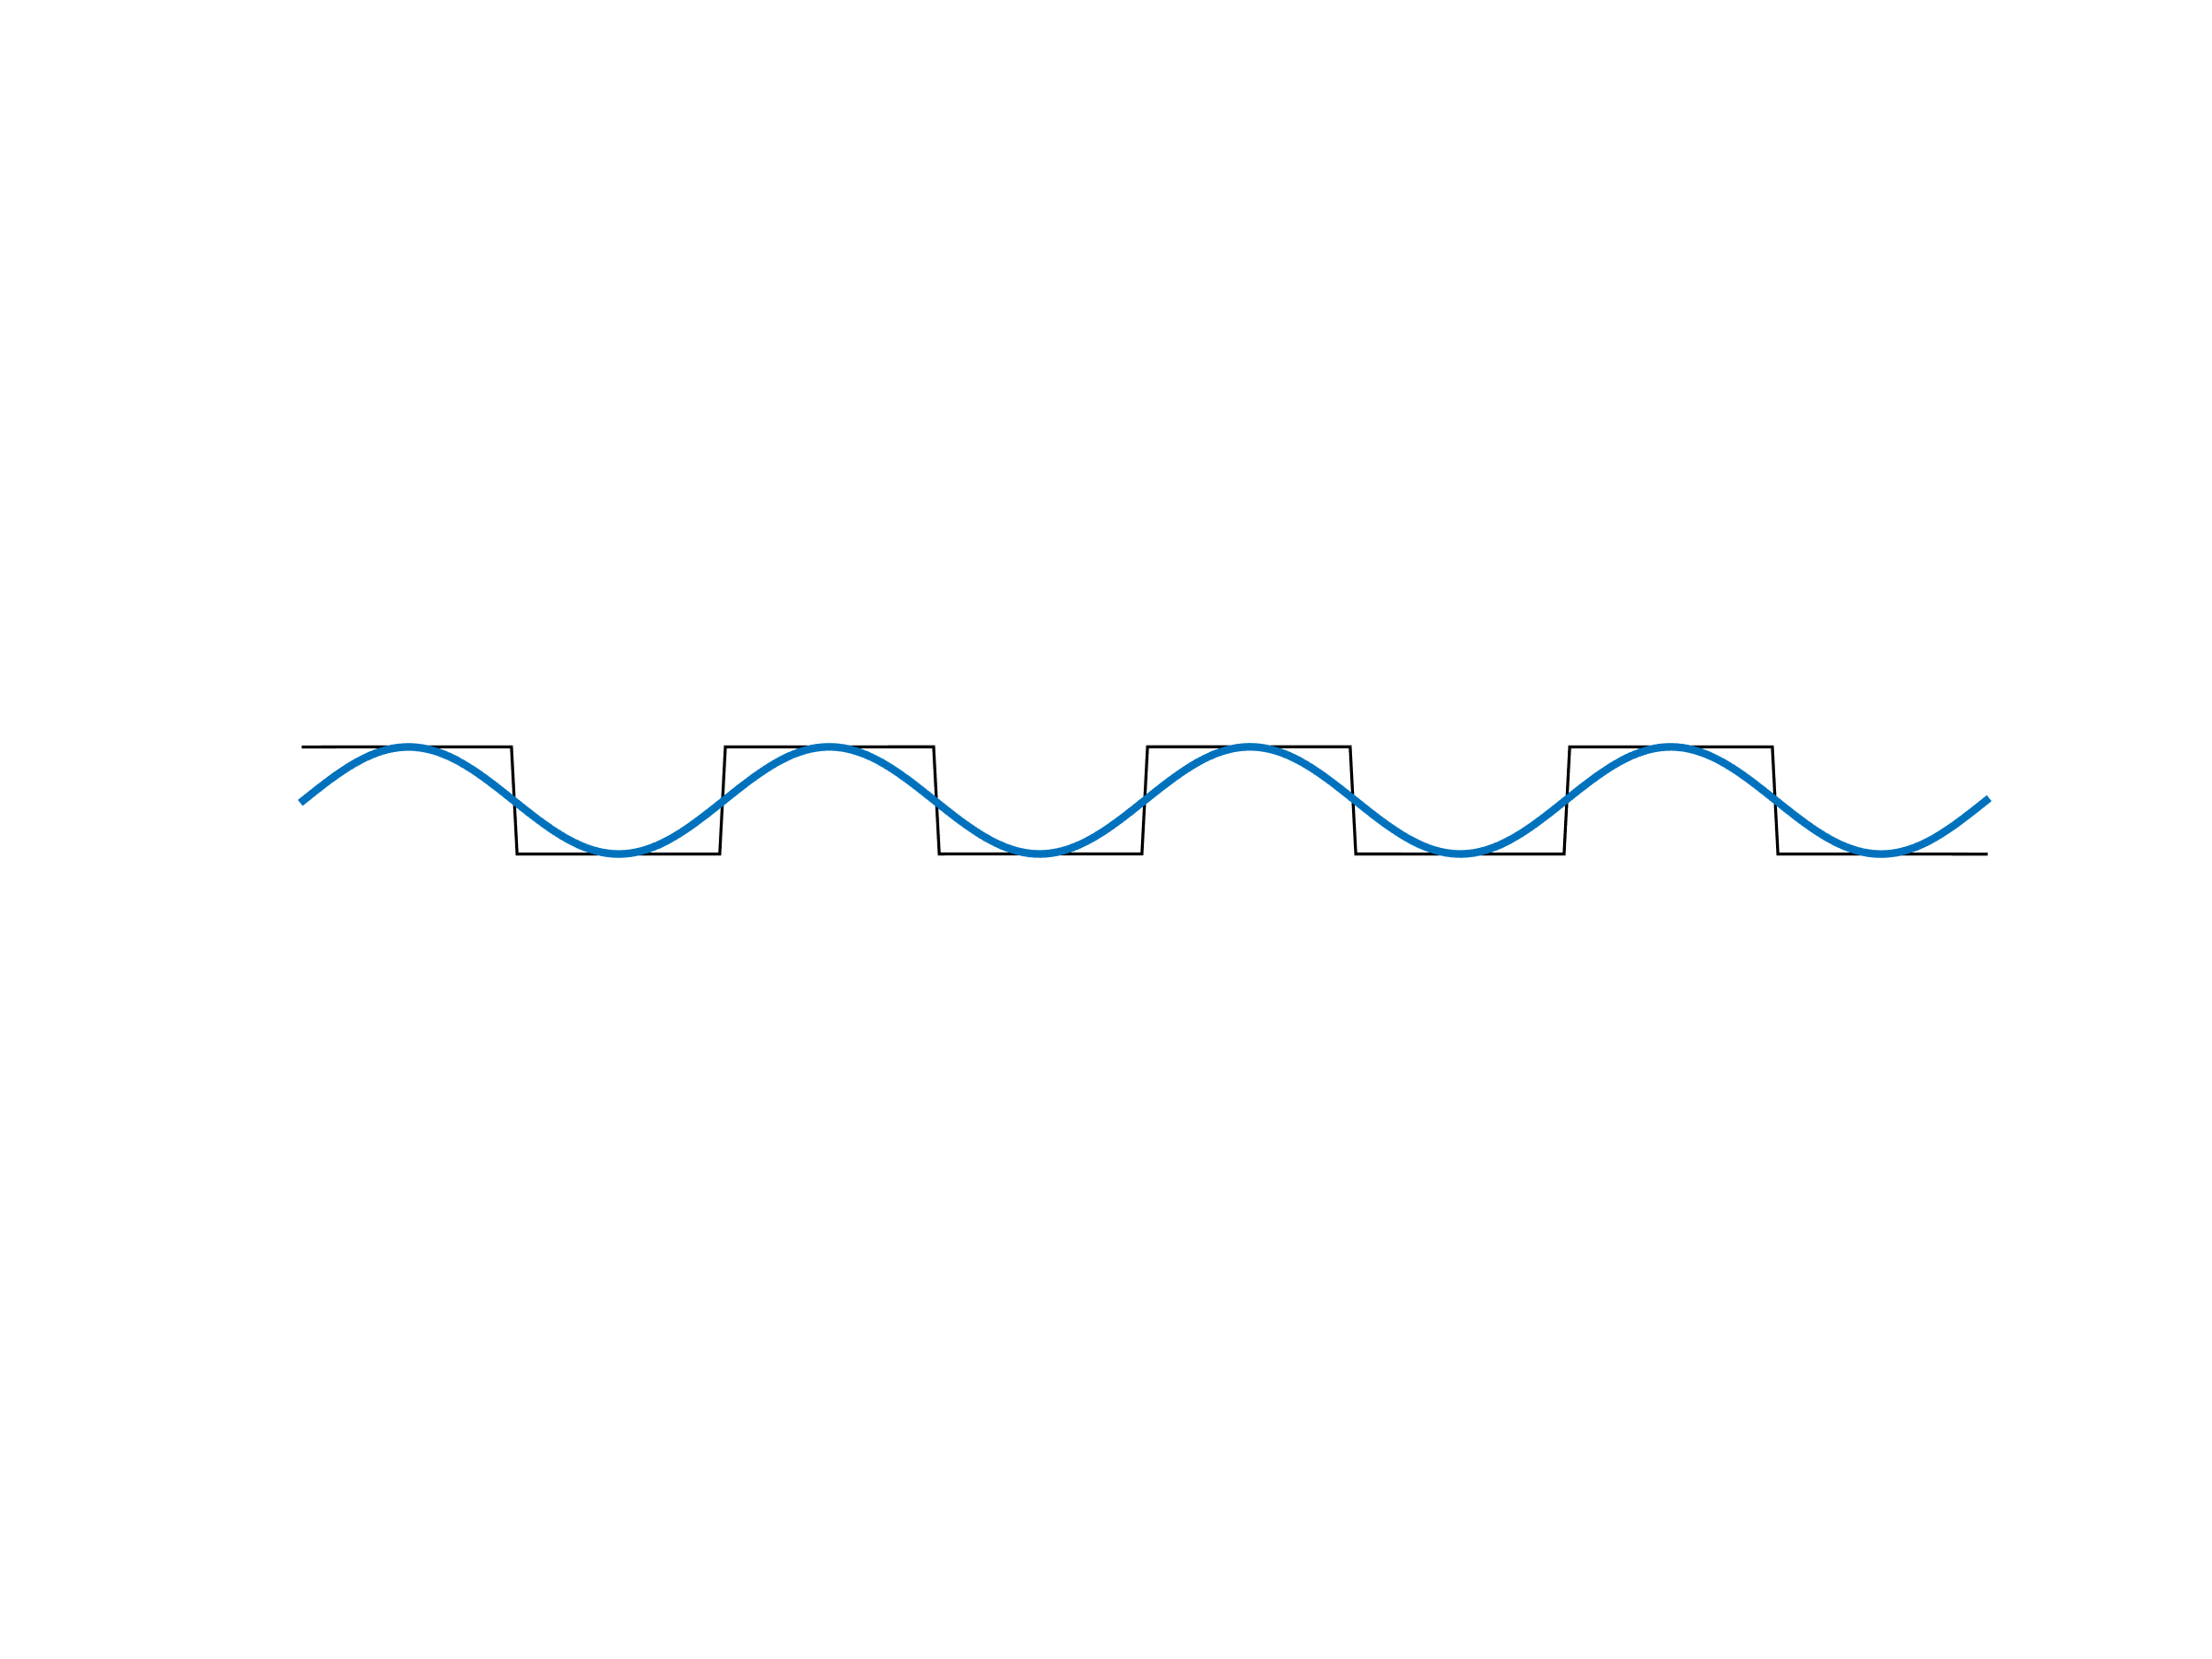
\includegraphics[width=2cm]{pic/markertrackerbendingstill1.png} 
%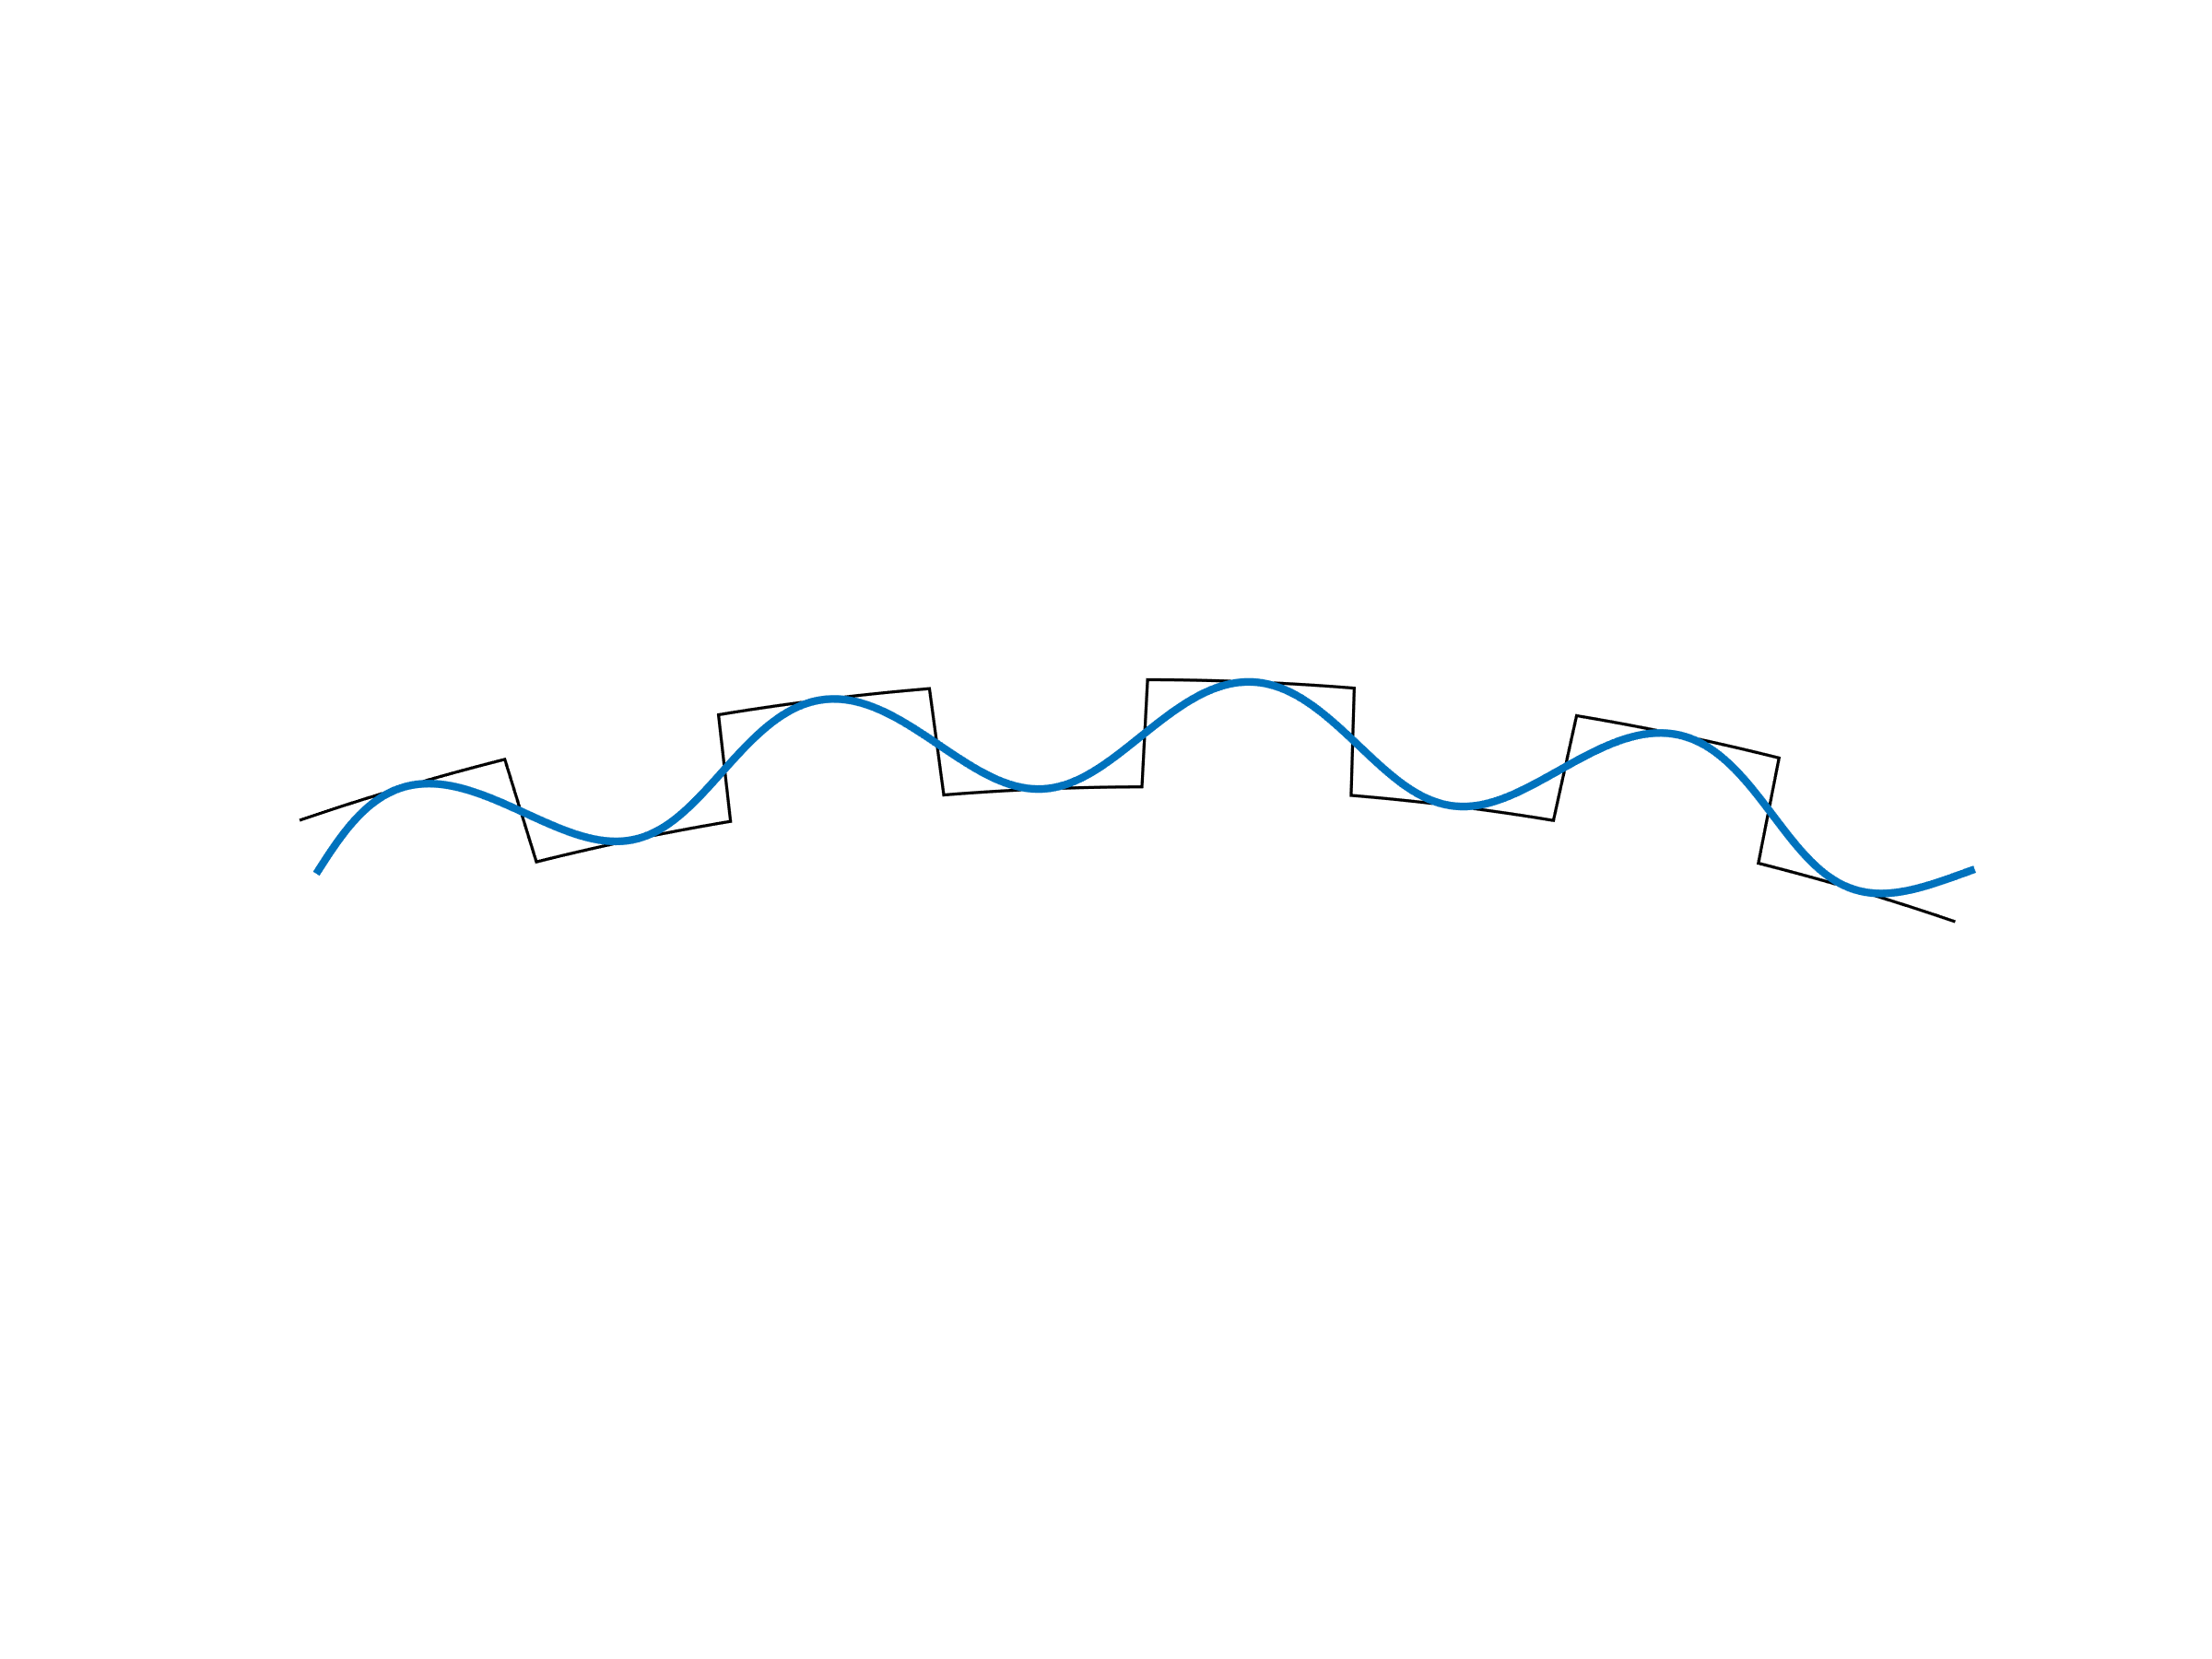
\includegraphics[width=2cm]{pic/markertrackerbendingstill61.png} 
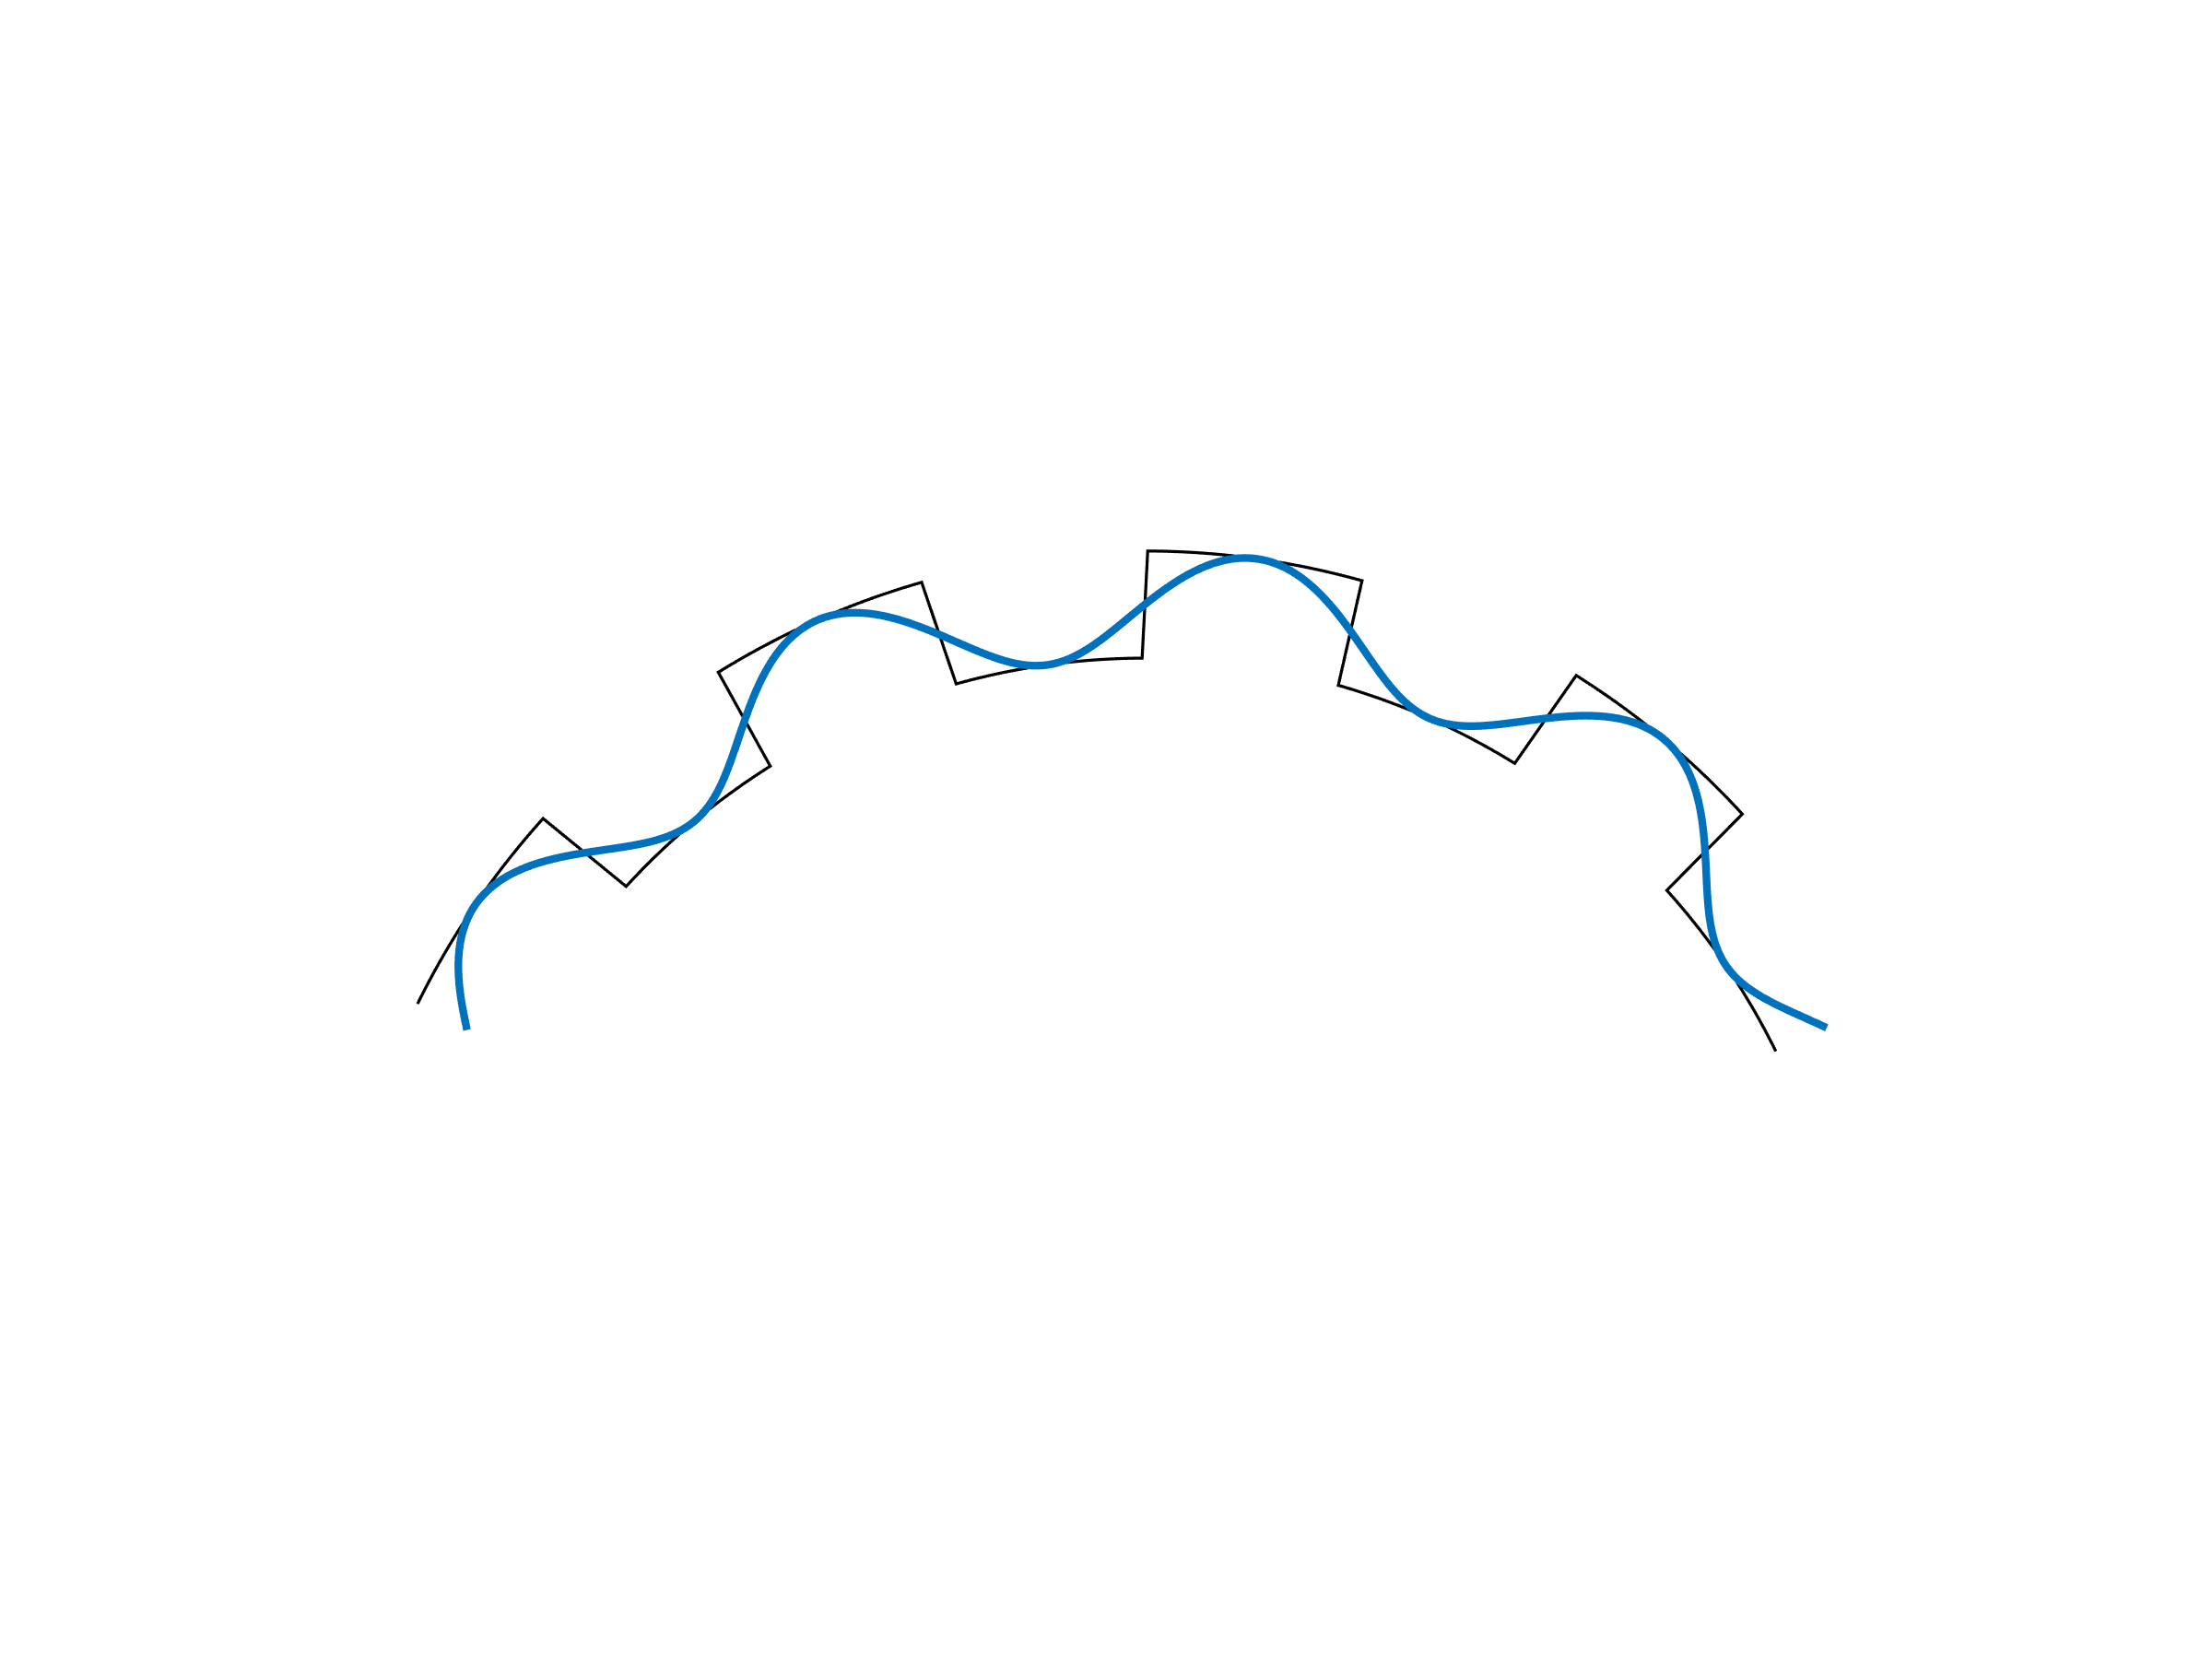
\includegraphics[width=2cm]{pic/markertrackerbendingstill121.png} 
%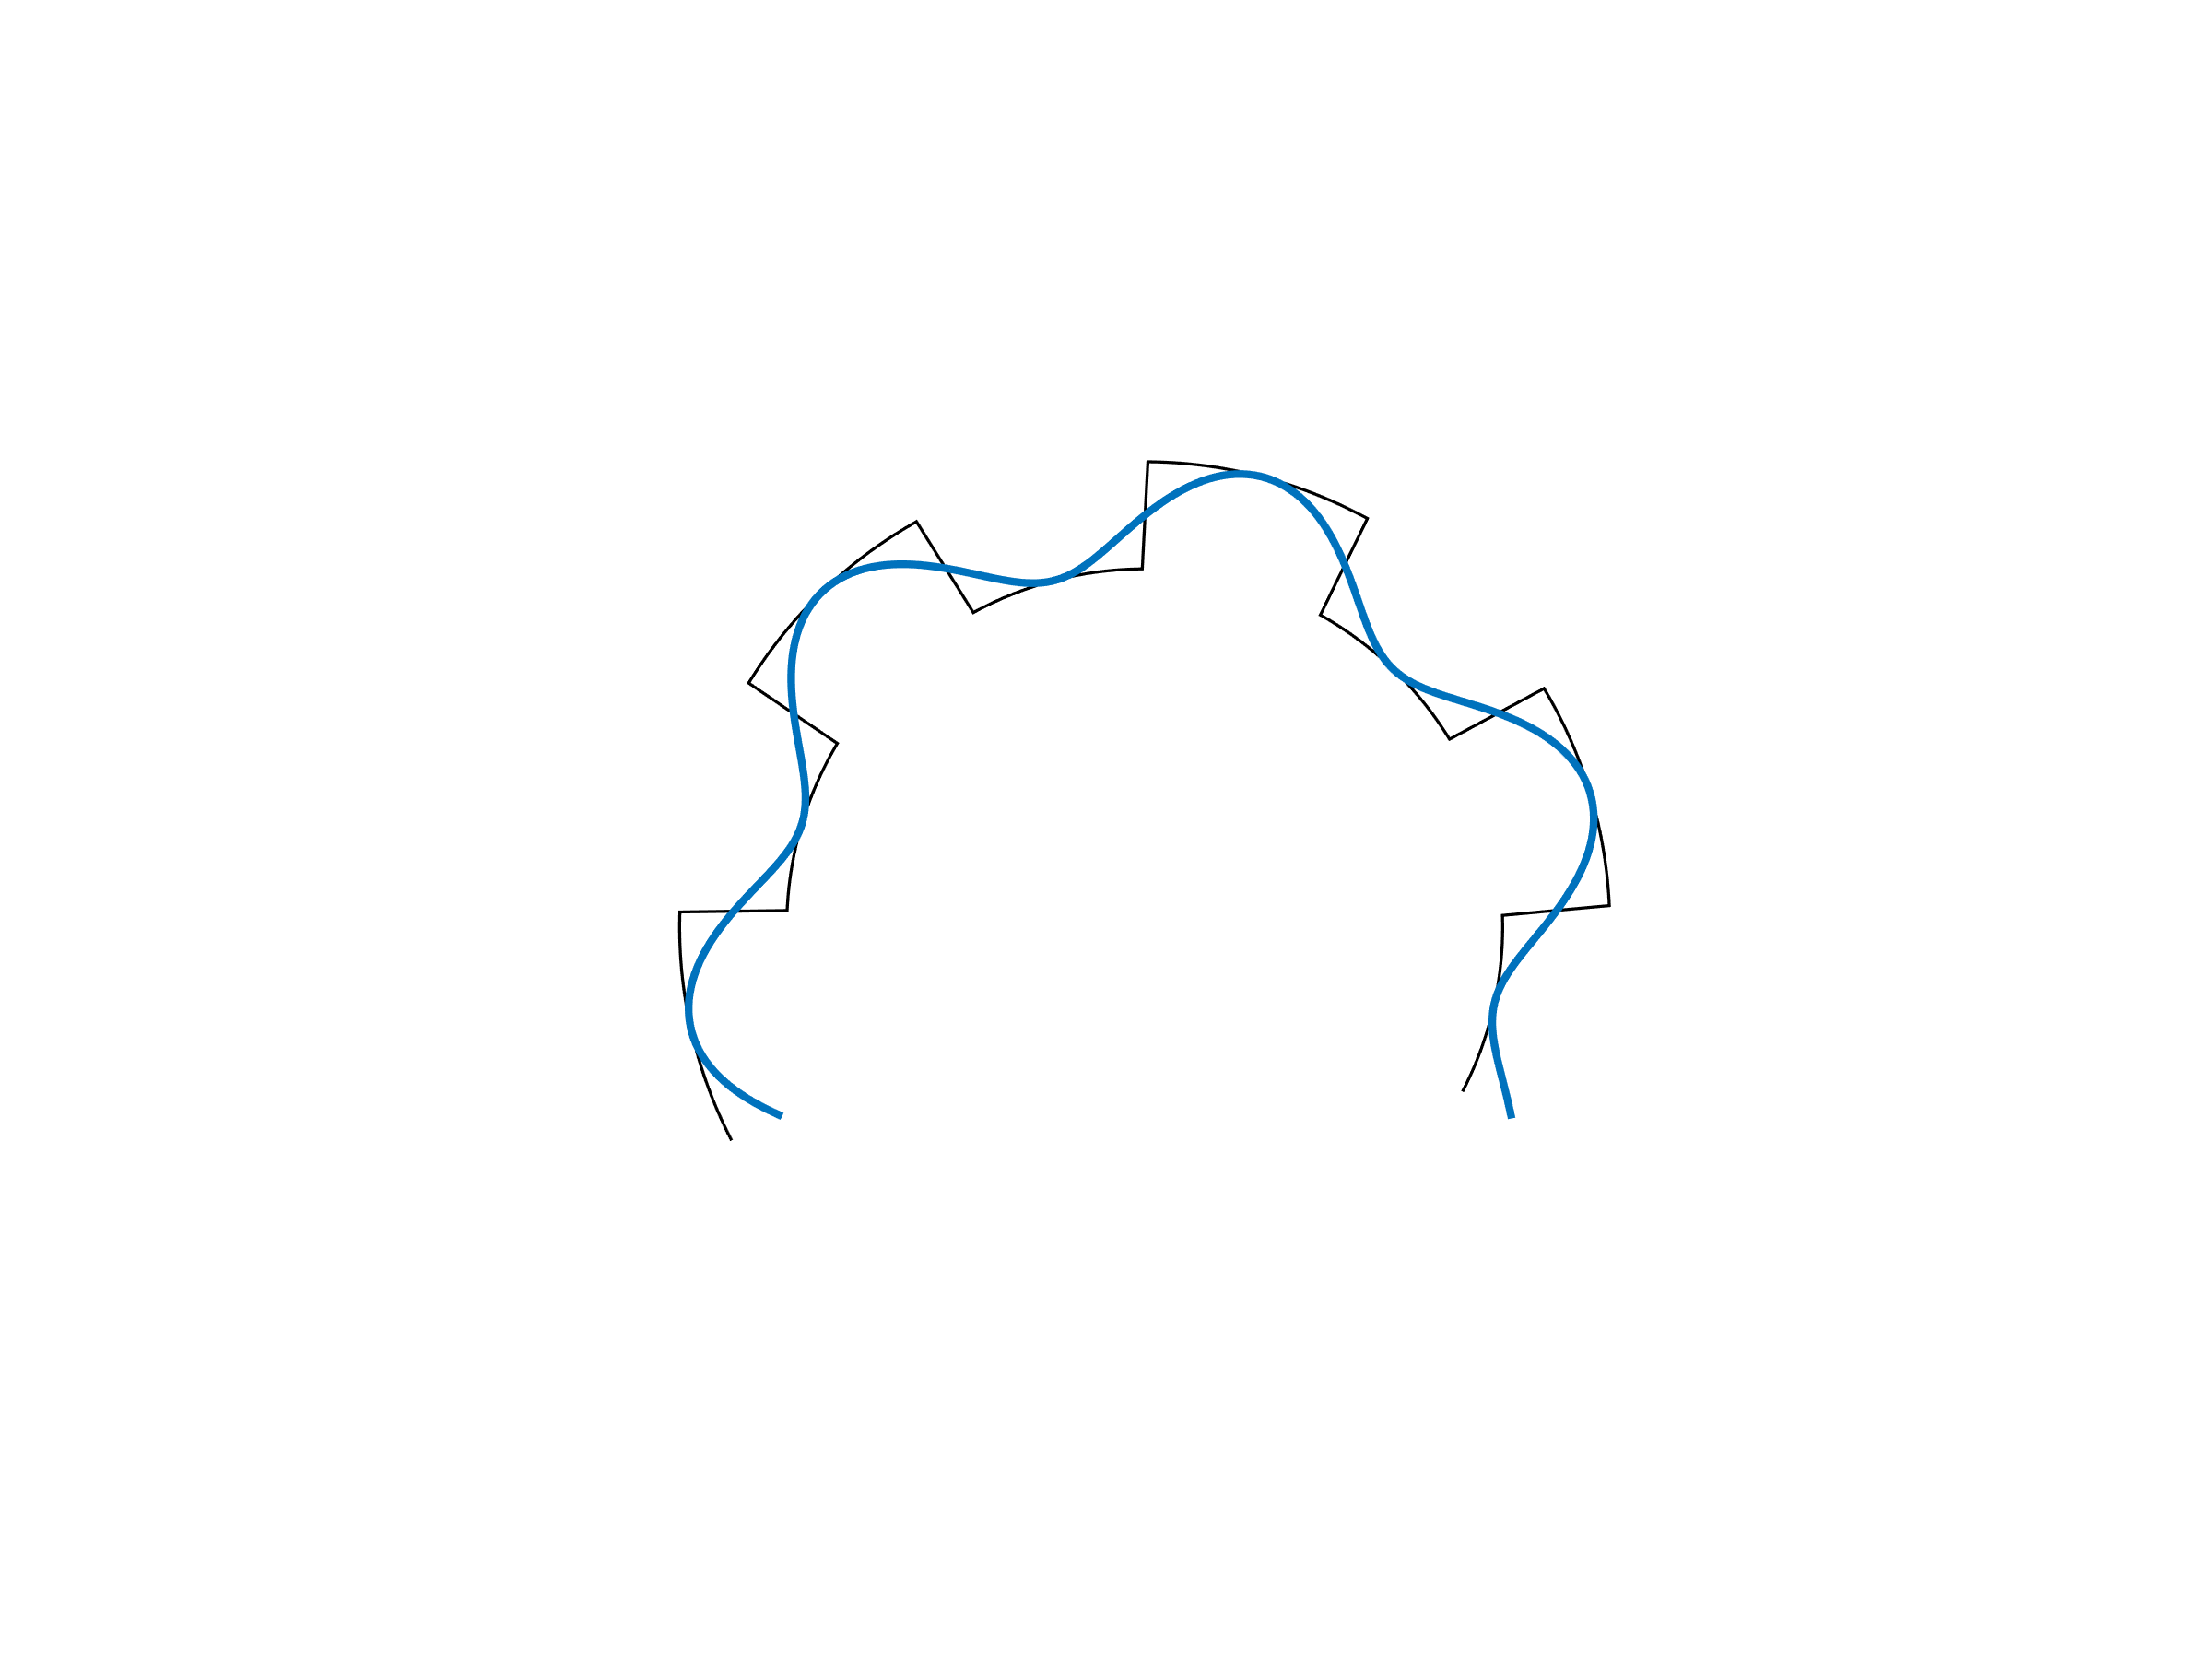
\includegraphics[width=2cm]{pic/markertrackerbendingstill181.png} 
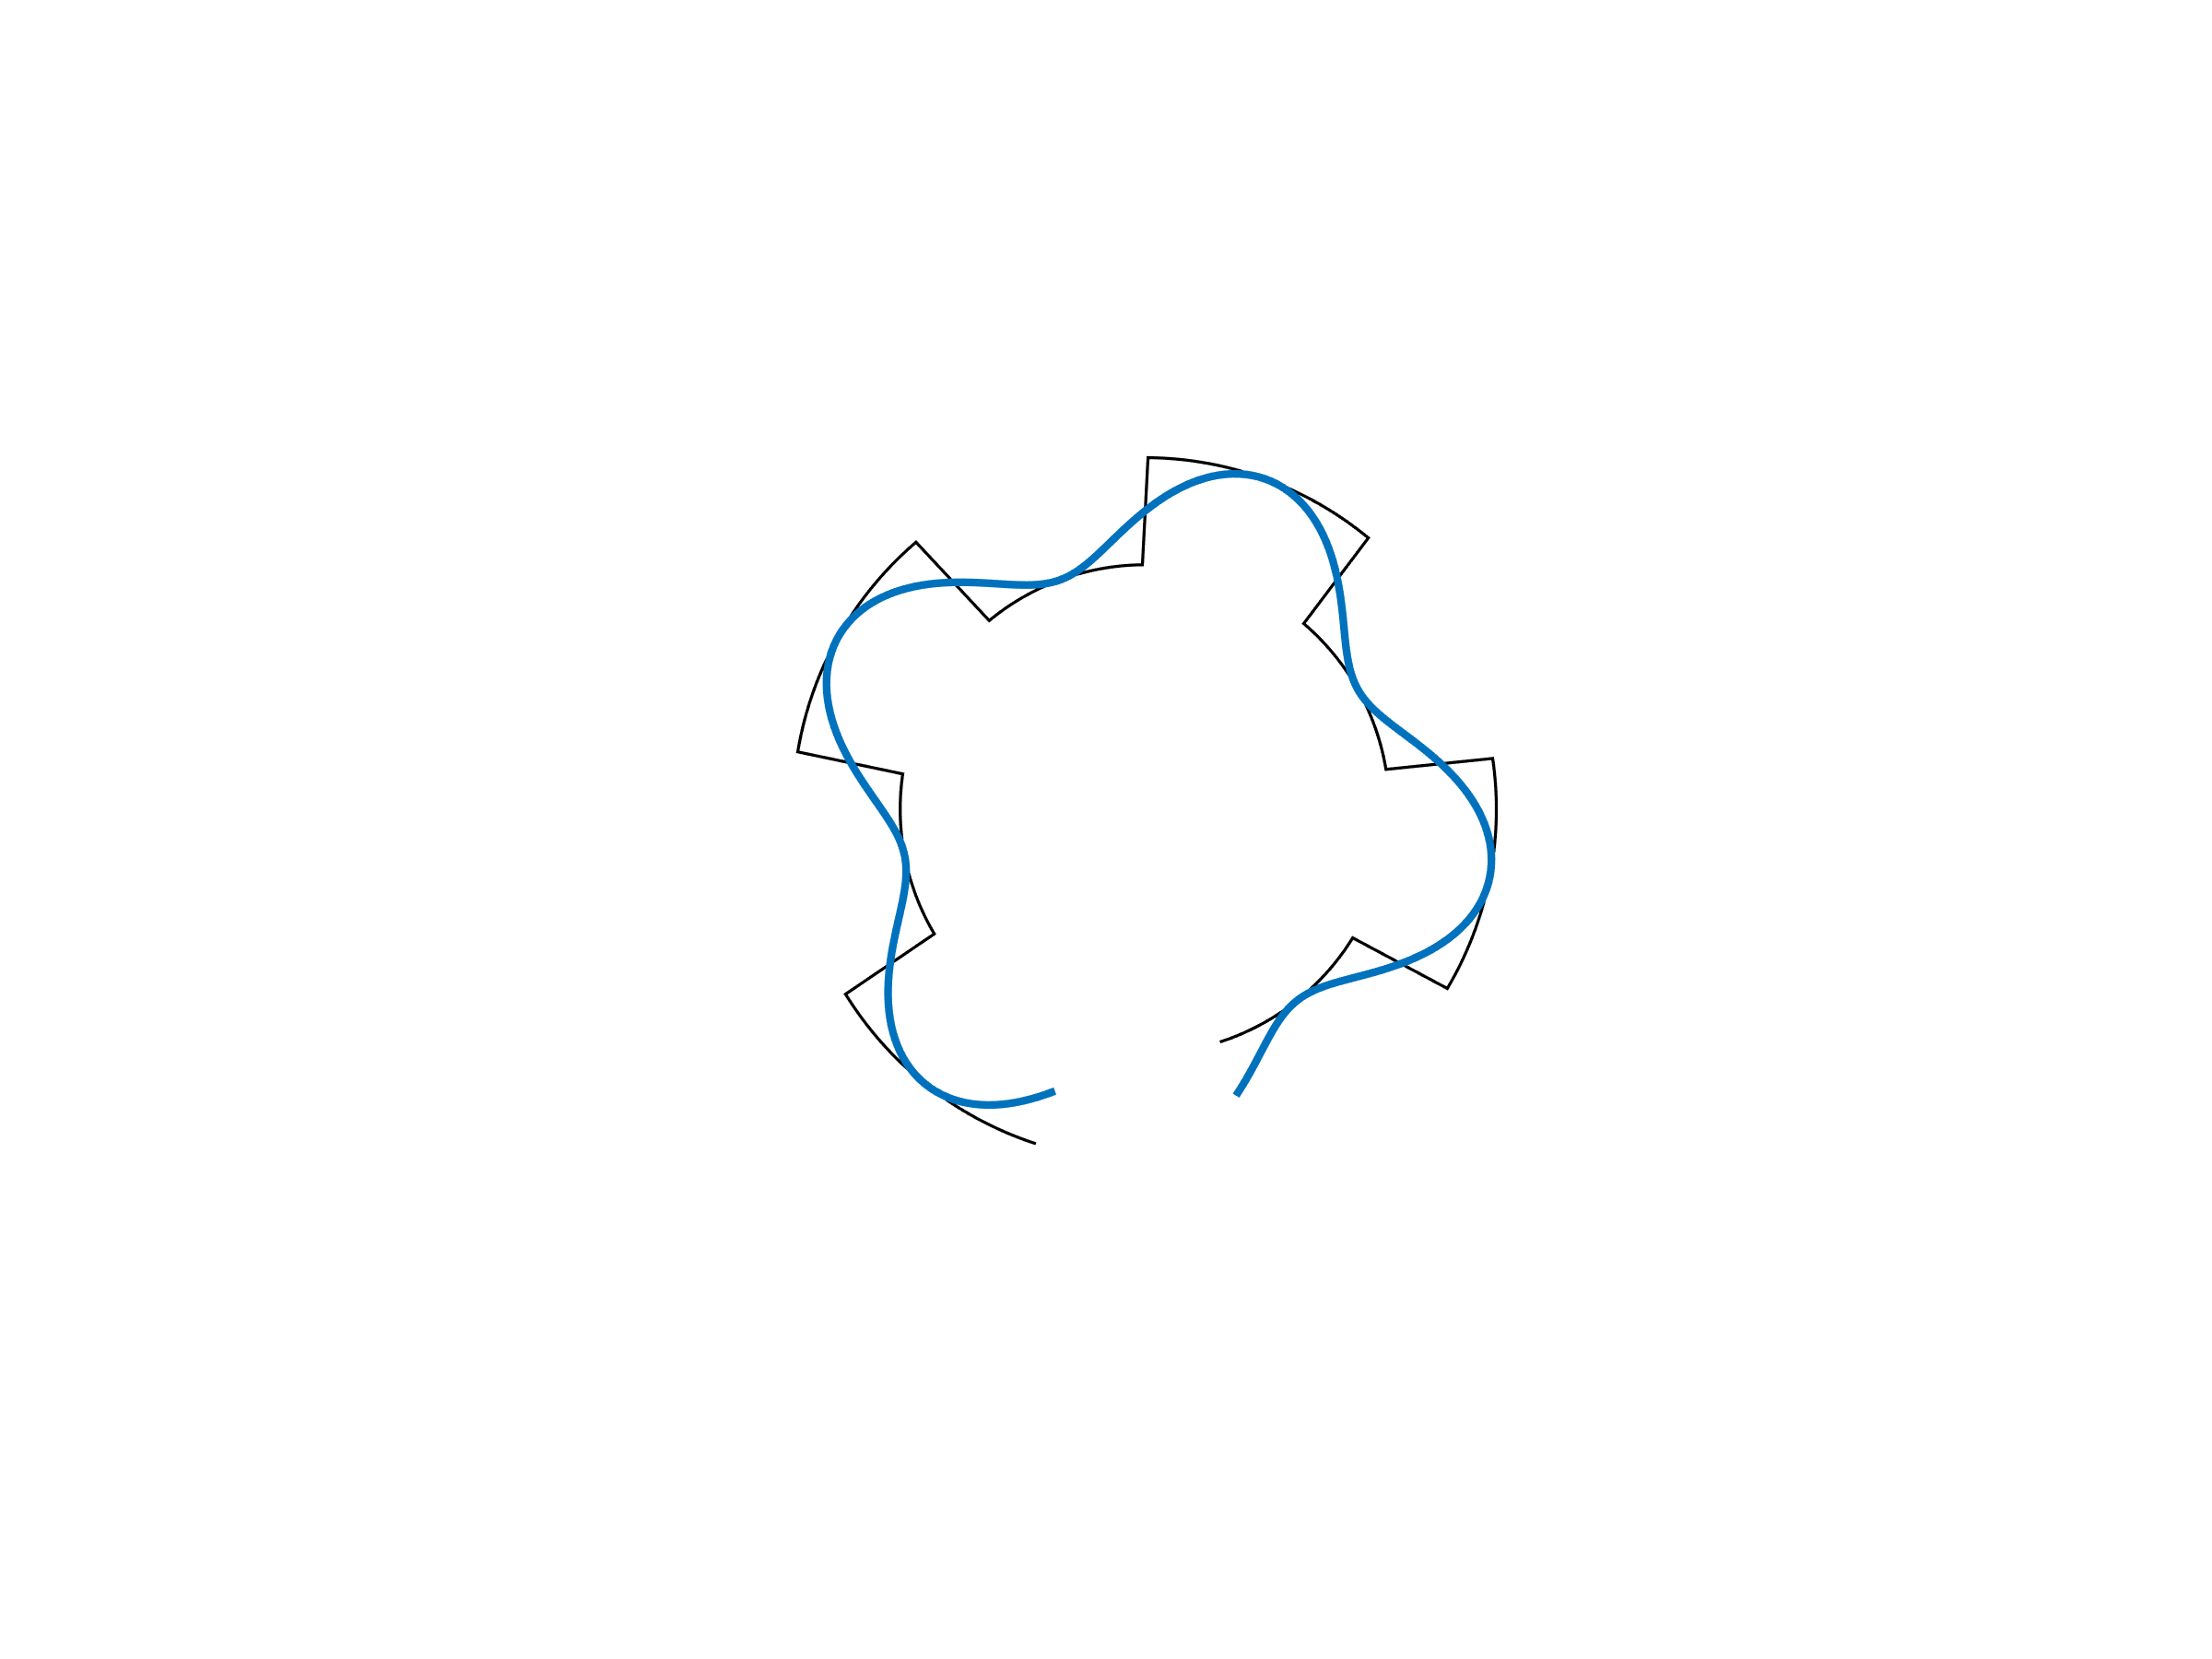
\includegraphics[width=2cm]{pic/markertrackerbendingstill241.png} 
%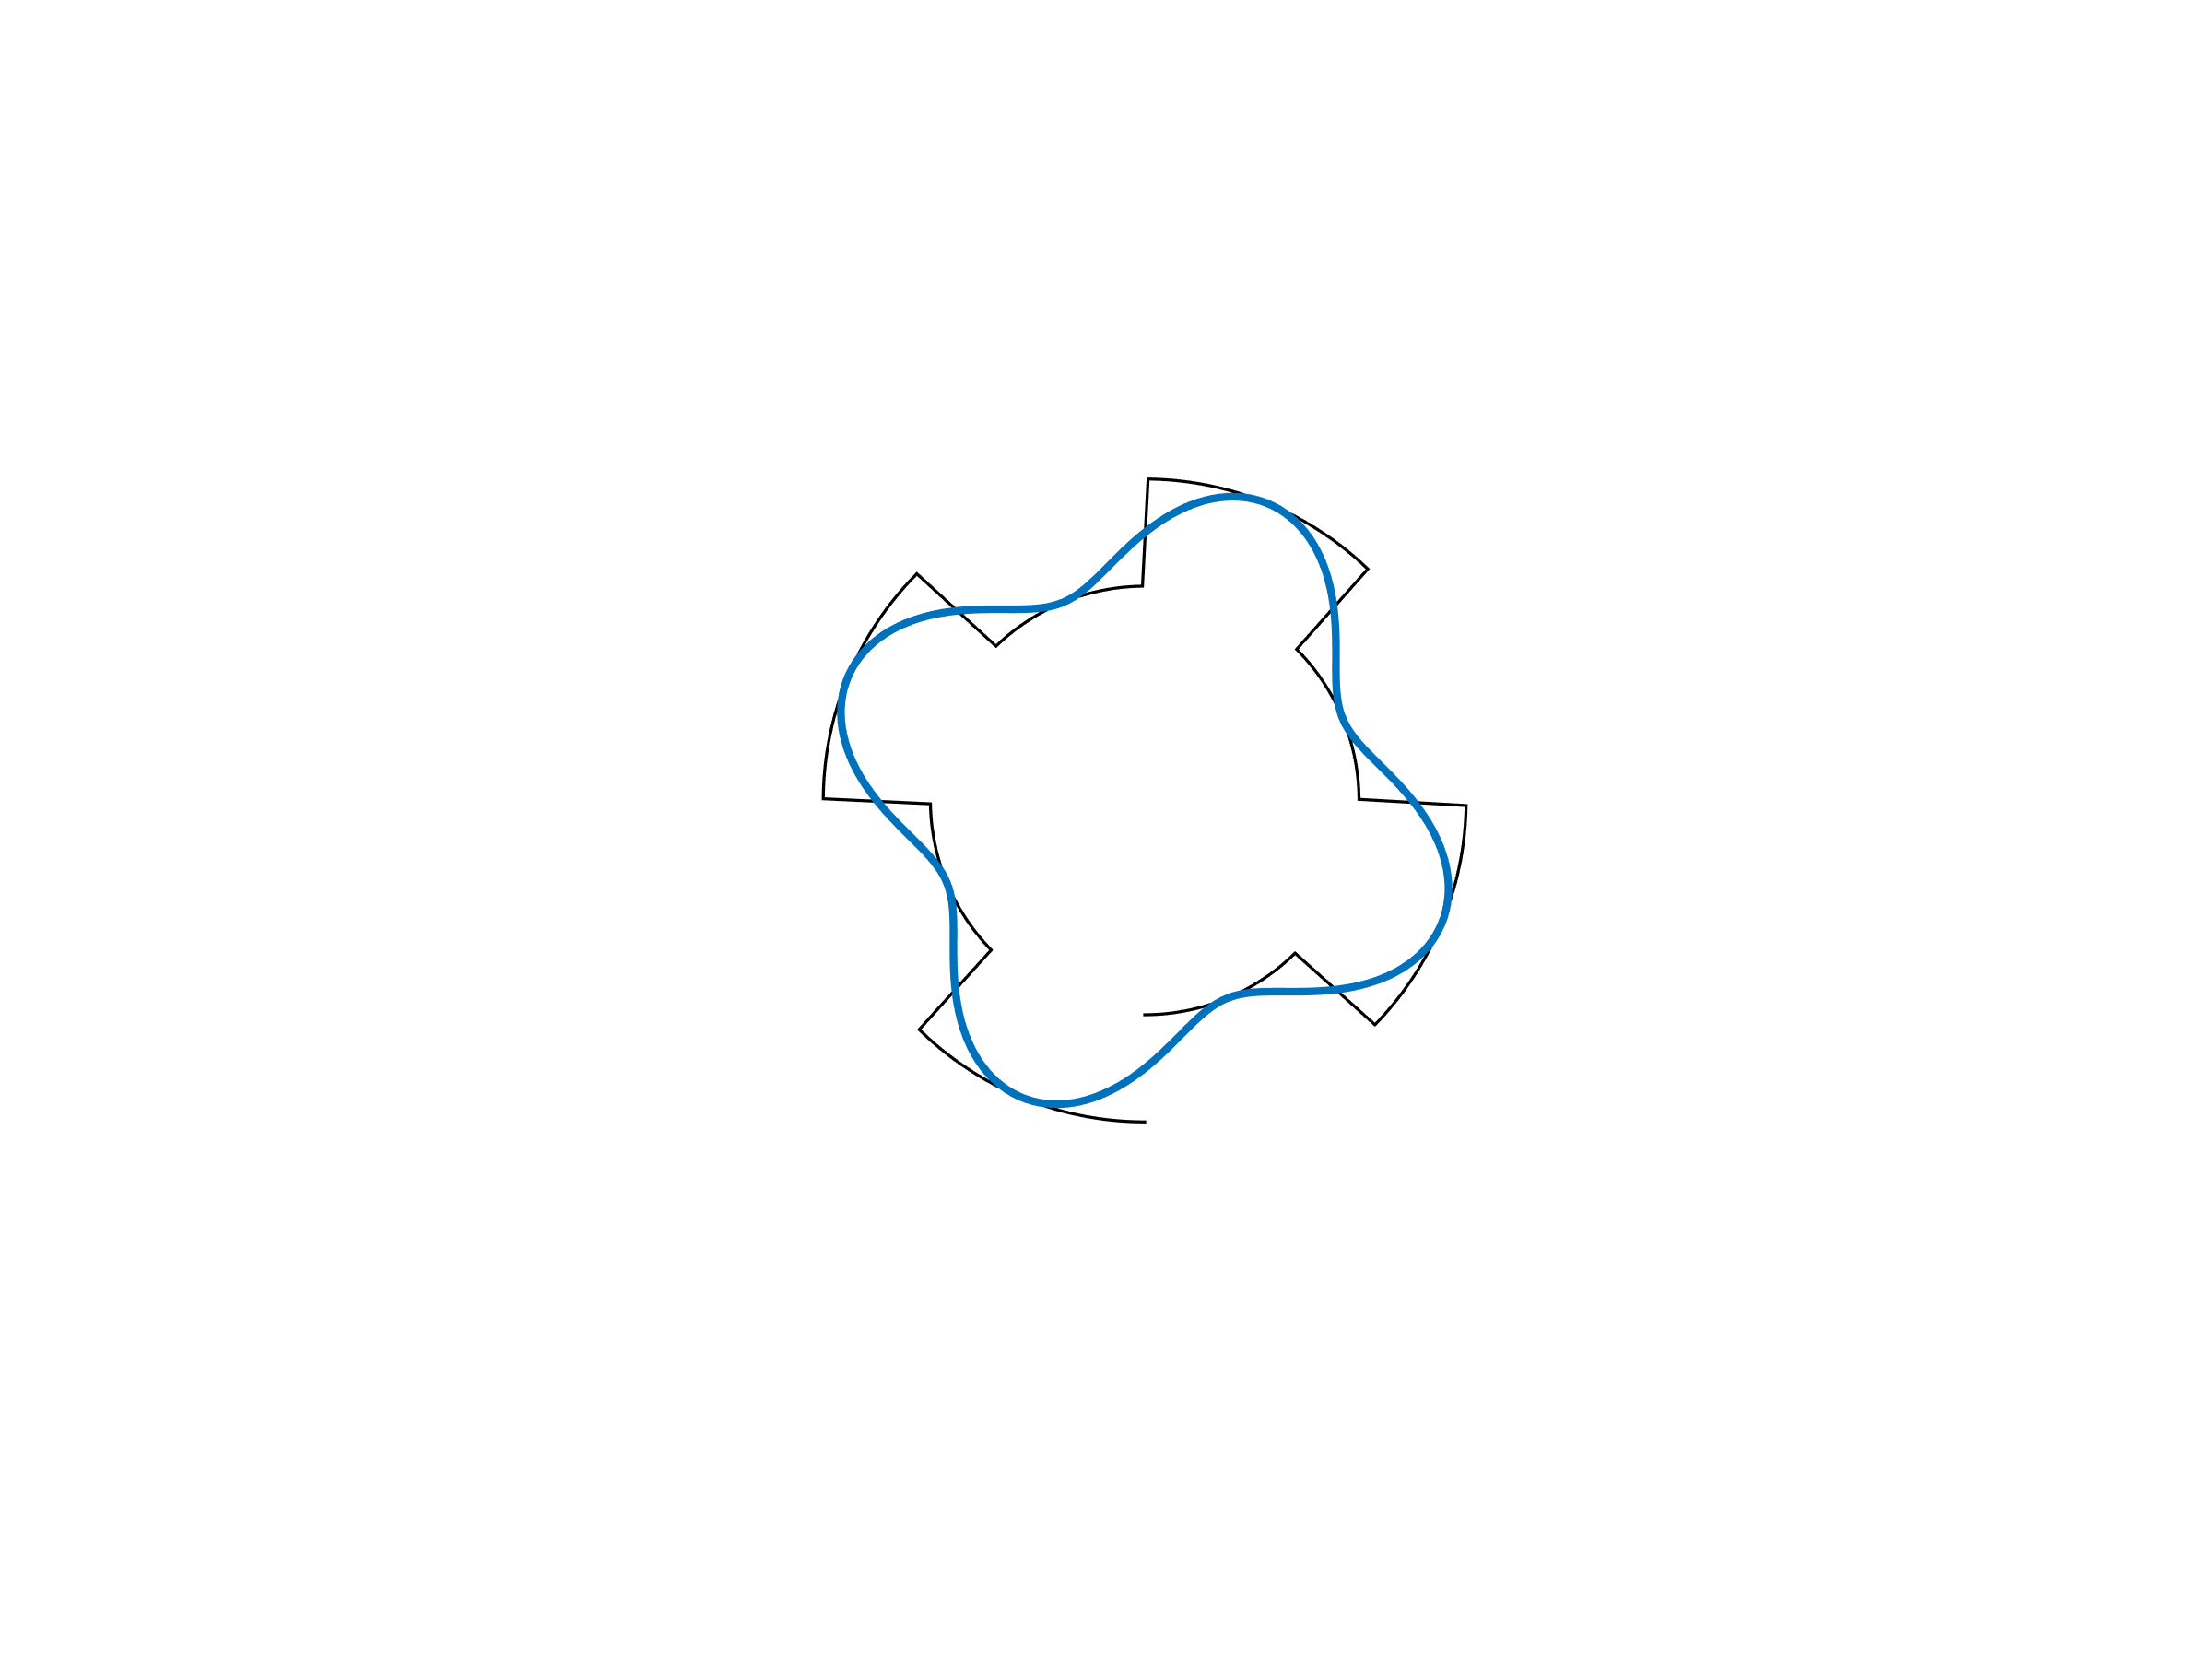
\includegraphics[width=2cm]{pic/markertrackerbendingstill300.png} 
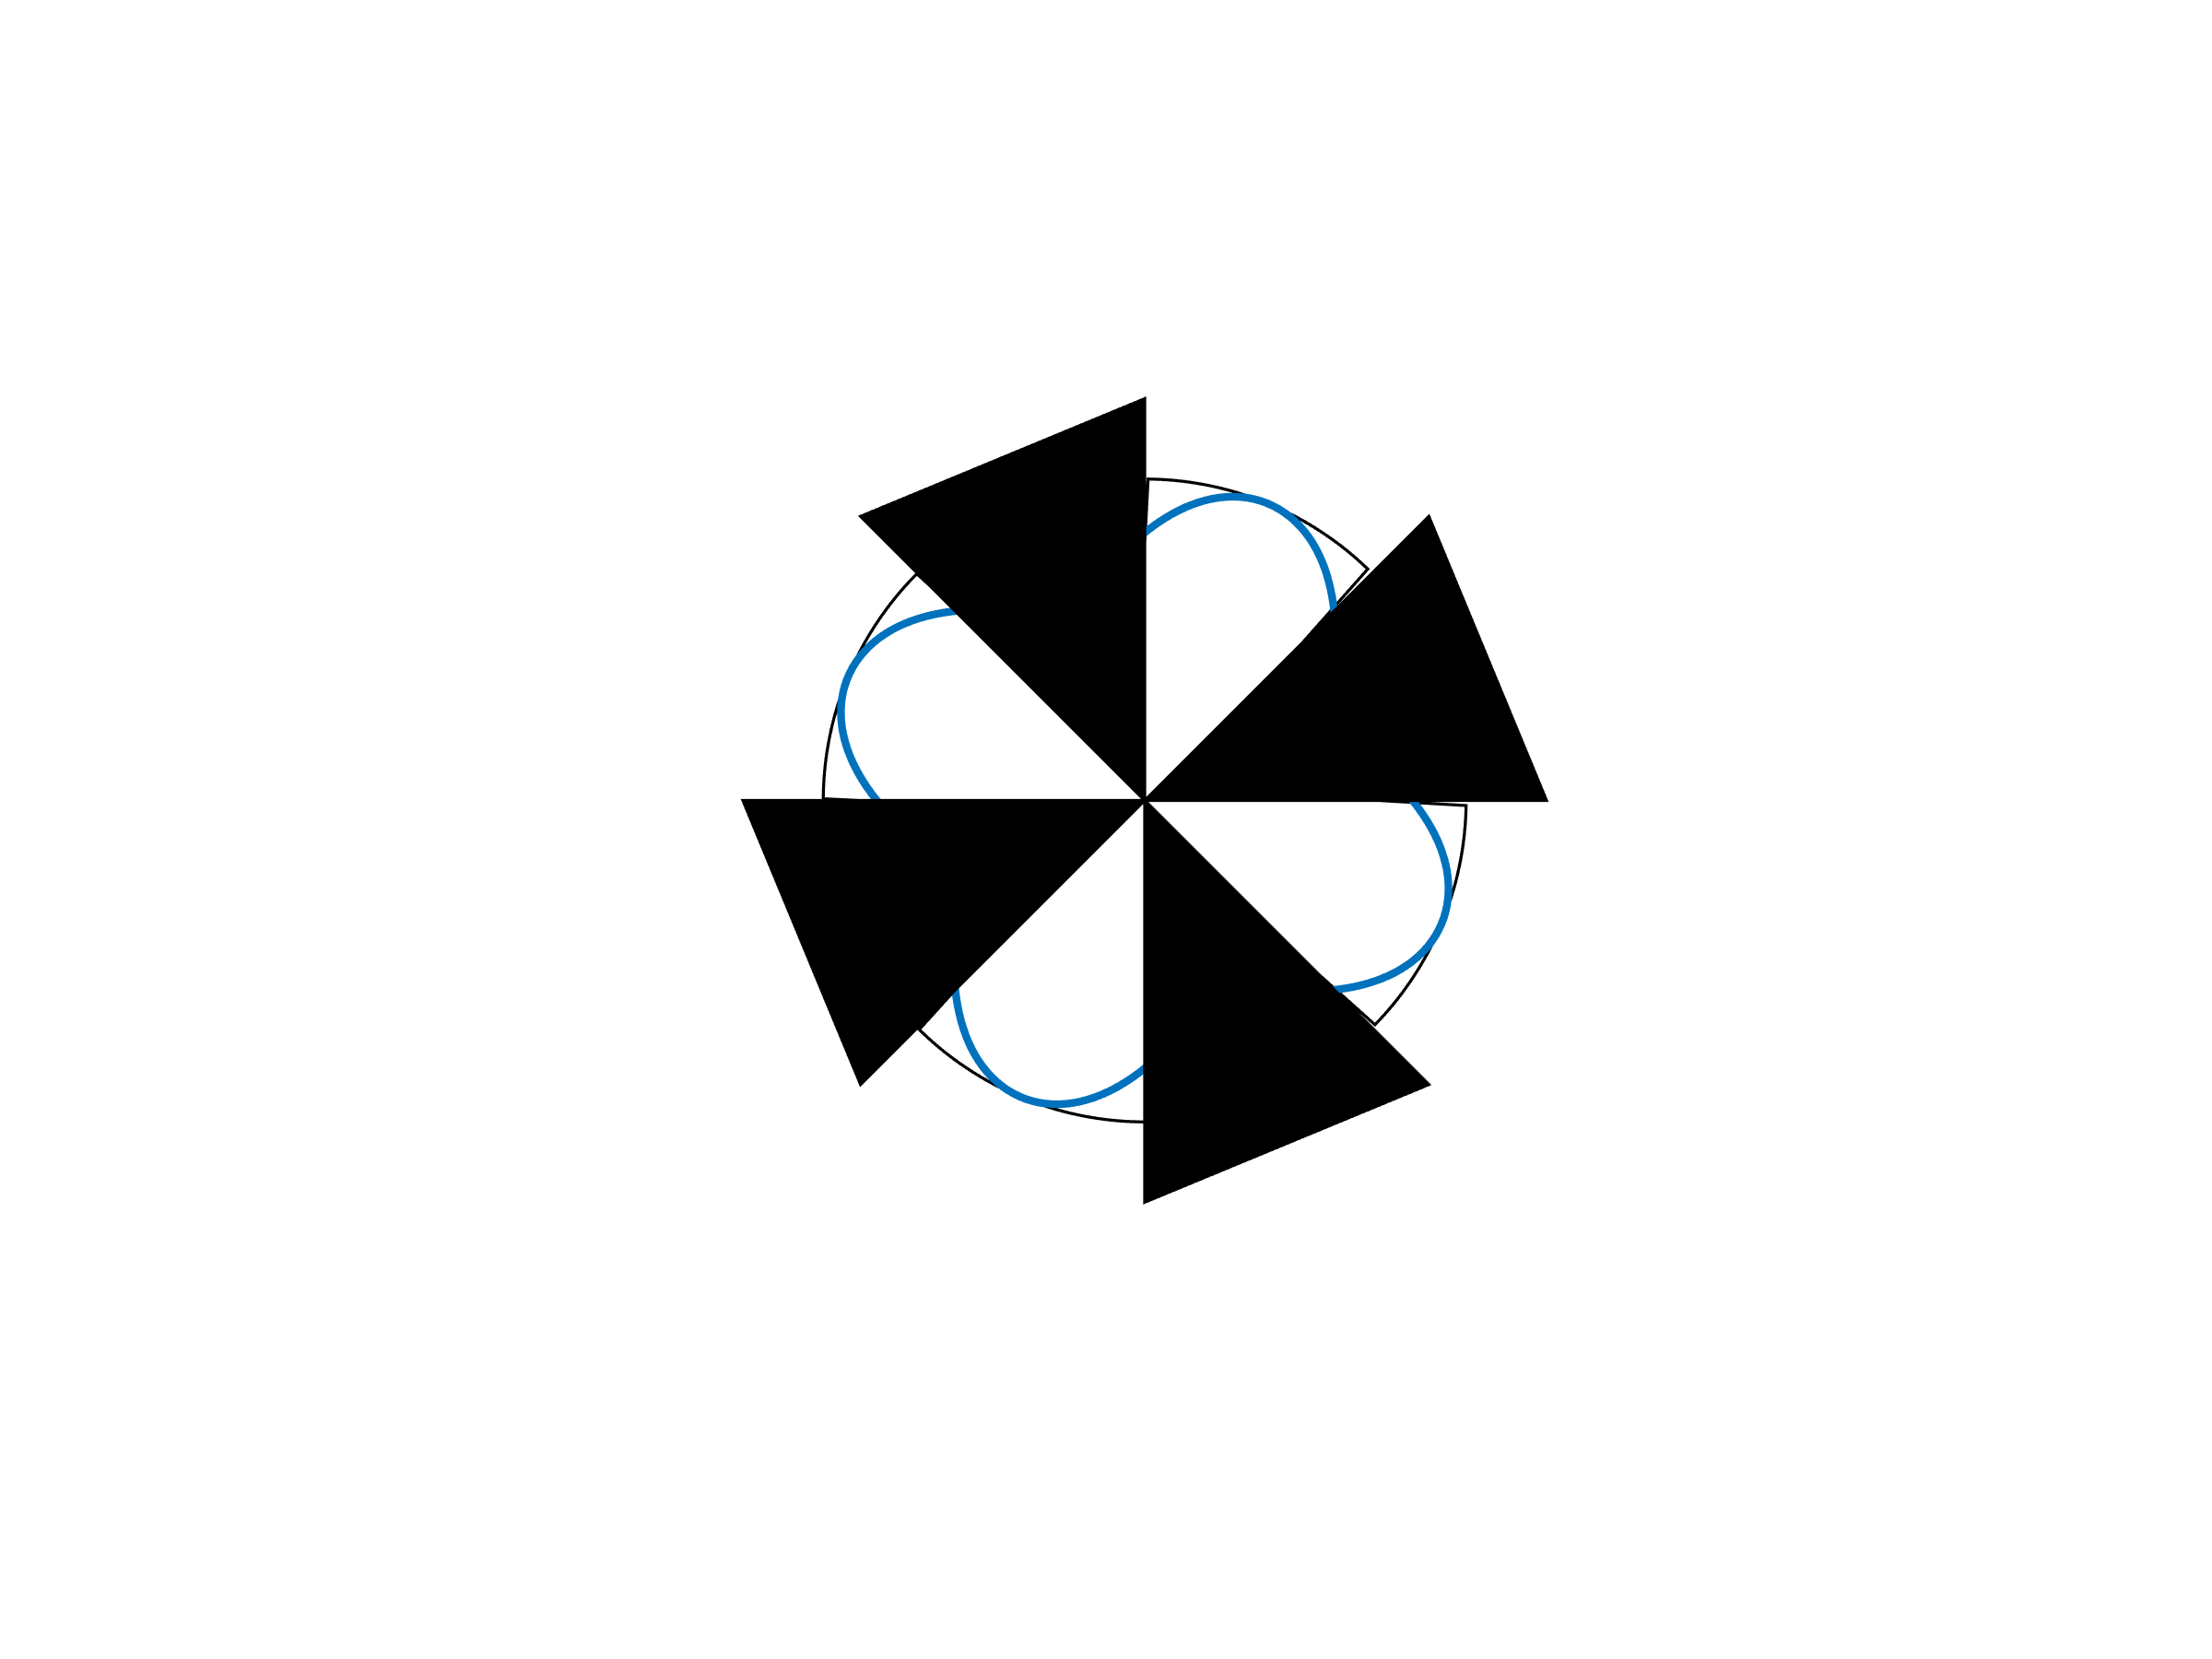
\includegraphics[width=3cm]{pic/finalmarker.png} 
\caption{Four repetitions of a square wave pattern is bent into a circular pattern around a central point. 
The direction from the central point out to the low levels of the square wave is coloured black.} 
\label{figBendingASquareWaveToACircularPattern} 
\end{figure} 
% node end (ID_1111025082)
% node start (ID_323744886)
% TEXT = Families of markers
By altering the number of repetitions of the black and white pattern around the central point, 
a set of different markers can be generated. 
The number of repetitions of the pattern is denoted the order ($n$) of the pattern. 
In figure \ref{figPlainMarkers} three patterns are visualised, the patterns have the orders 
$n = 2$, $n = 3$ and $n = 4$. 
% node end (ID_323744886)
% node start (ID_1460525345)
% TEXT = figPlainMarkers
\begin{figure} 
\newcommand{\steplength}{30} 
\newcommand{\archlength}{1.6cm} 
\newcommand{\drawarch}[1]{\draw[color=black,fill=black] (2*#1:\archlength) arc(2*#1:2*#1+\steplength:\archlength) 
-- (0, 0) -- (2*#1:\archlength); } 
%\newcommand{\drawdot}{\draw[fill=black] (0, 0) circle (0.75mm);} 
\newcommand{\drawdot}{} 
\newcommand{\draworder}[1]{\draw (0, -2.2) node {n = #1};} 
\renewcommand{\archlength}{1cm} 
\begin{tikzpicture} 
\newcommand\order{2} 
\begin{scope} 
% Do calculation 
\pgfmathsetmacro{\steplength}{180 / \order}% 
\foreach \n in {0, \steplength, ..., 179}{\drawarch{\n}} 
\end{scope} 
\renewcommand\order{3} 
\begin{scope}[xshift=3.5cm] 
% Do calculation 
\pgfmathsetmacro{\steplength}{180 / \order}% 
\foreach \n in {0, \steplength, ..., 179}{\drawarch{\n}} 
\end{scope} 
\renewcommand\order{4} 
\begin{scope}[xshift=2*3.5cm] 
% Do calculation 
\pgfmathsetmacro{\steplength}{180 / \order}% 
\foreach \n in {0, \steplength, ..., 179}{\drawarch{\n}} 
\end{scope} 
\renewcommand\order{5} 
\begin{scope}[xshift=3*3.5cm] 
% Do calculation 
\pgfmathsetmacro{\steplength}{180 / \order}% 
\foreach \n in {0, \steplength, ..., 179}{\drawarch{\n}} 
\end{scope} 
\end{tikzpicture} 
\caption{Markers with different orders ($n = 2 \ldots 5$).} 
\label{figPlainMarkers} 
\end{figure} 
% node end (ID_1460525345)
% node start (ID_1931572391)
% TEXT = Detection of a marker
\subsection{Detection of a marker} 
% node end (ID_1931572391)
% node start (ID_166592580)
% TEXT = Use a convolution to detect a certain square wave
Detection of a square wave with $n$ repetitions using Fourier analysis, 
relies on a convolution of the $N$ measurement of the signal with the kernel $Y_n$: 
\[ 
Y_n = e^{-i 2 \pi k n / N} \qquad k \in [0, \ldots, N - 1] 
\] 
% node end (ID_166592580)
% node start (ID_1719695254)
% TEXT = Use a convolution to detect an n-fold edge
A somewhat similar kernel is used to detect the n-fold edge markers. 
The kernel is specified using polar coordinates as follows: 
\[ 
Z_n = e^{-i n \theta} \cdot r^n \cdot e^{-8 r^2} 
\] 
where $\theta$ is the direction and $r$ is the distance to the actual position in the kernel. 
The center of the polar coordinates are placed in the middle of the kernel and 
is scaled such that a circle with radius 1 is the largest circle that can be placed inside the kernel. 
Four different views of a kernel with order $n = 4$ is shown in 
figure \ref{figKernelToDetectPlainMarker}. 
 
% node end (ID_1719695254)
% node start (ID_715171165)
% TEXT = figKernelToDetectPlainMarker
\begin{figure} 
\begin{subfigure}[t]{0.46\textwidth} 
\includegraphics[width=4cm]{matlabpic/kernelRealPart.png} 
\caption{Real part of kernel.} 
\label{figRealPartOfN4Kernel} 
\end{subfigure} 
\begin{subfigure}[t]{0.46\textwidth} 
\includegraphics[width=4cm]{matlabpic/kernelImagPart.png} 
\caption{Imaginary part of kernel.} 
\label{figImagPartOfN4Kernel} 
\end{subfigure} 
\begin{subfigure}[t]{0.46\textwidth} 
\includegraphics[width=4cm]{matlabpic/kernelAbs.png} 
\caption{Magnitude of kernel.} 
\label{figMagnitudeOfN4Kernel} 
\end{subfigure} 
\begin{subfigure}[t]{0.46\textwidth} 
\includegraphics[width=4cm]{matlabpic/kernelArg.png} 
\caption{Argument of kernel.} 
\label{figArgumentOfN4Kernel} 
\end{subfigure} 
\caption{Different views of the complex kernel used for detecting n-fold markers ($n = 4$).} 
\label{figKernelToDetectPlainMarker} 
\end{figure} 
% node end (ID_715171165)
% node start (ID_26878778)
% TEXT = Detecting the marker
To detect a marker with a known order, the input image is converted to a grayscale image and then convolved with the $Z_n$ kernel. 
As the $Z_n$ kernel contains complex weights, the resulting image will contain complex values. 
The magnitude of the complex values in the resulting image, tells us how well the 
input picture matches the used kernel, this is visualised in figure \ref{figDetectionExample}; 
the argument of the complex value tells the orientation of the 
pattern, to best match the input image. 
% node end (ID_26878778)
% node start (ID_949098152)
% TEXT = figDetectionExample
\begin{figure} 
\begin{subfigure}[t]{0.46\textwidth} 
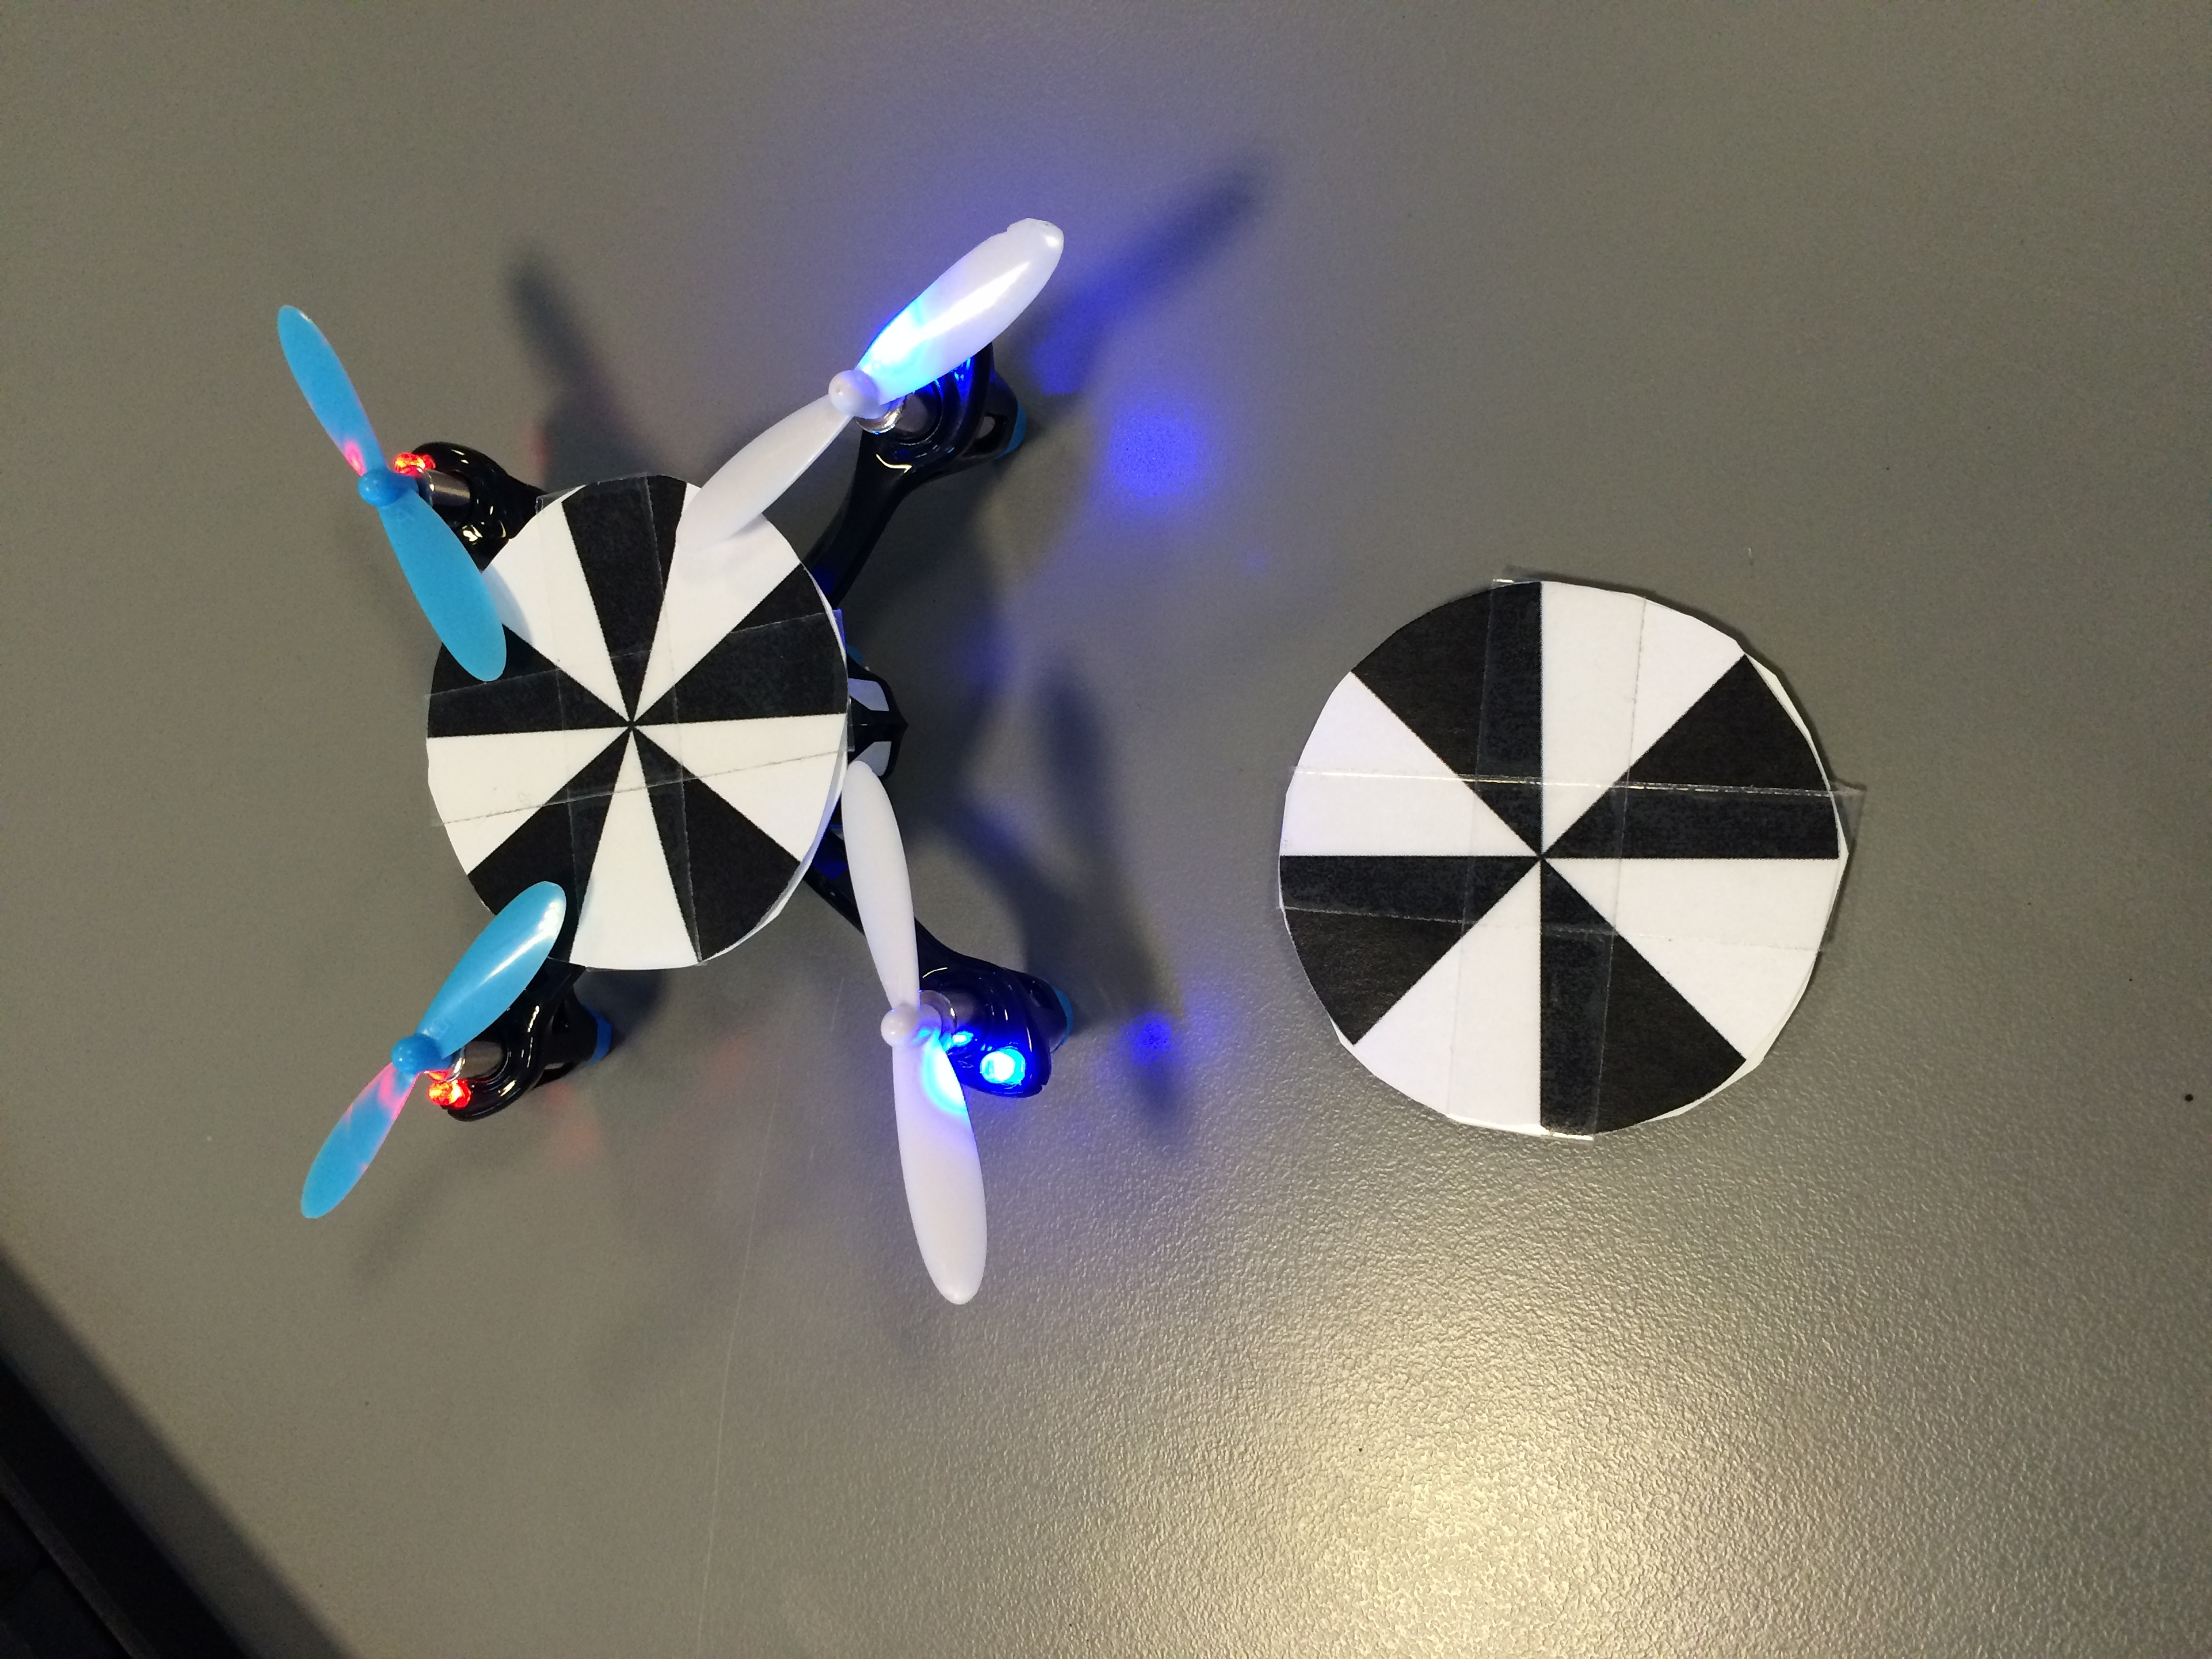
\includegraphics[width=5cm]{matlabpic/hubsanwithmarker.jpg} 
\caption{Input image containing markers of order 4 and 5.} 
\label{figHubsanInputImage} 
\end{subfigure} 
\begin{subfigure}[t]{0.46\textwidth} 
\includegraphics[width=5cm]{matlabpic/scaledmarkerresponseinverted.png} 
\caption{Marker detection response in inverted colors. Black denotes a high response to the marker.} 
\label{figHubsanMarkerDetectionReponse} 
\end{subfigure} 
\caption{Marker detection example response.} 
\label{figDetectionExample} 
\end{figure} 
% node end (ID_949098152)
% node start (ID_1005629562)
% TEXT = Quality estimate of detected marker
\subsection{Estimating the quality of the detected marker} 
% node end (ID_1005629562)
% node start (ID_1644690044)
% TEXT = Issue with markers with different orders
Interpreting the magnitude response to the $Z_n$ kernel poses an issue 
when markers with different (but nearby) orders are present in the input image. 
As can be seen in figure \ref{figDetectionExample}, where a marker of order $n = 4$ 
is being detected, there is a moderate response around the marker mounted on the Hubsan UAV with order $n = 5$. 
This issue can of course be reduced by avoiding markers with similar orders in the same image, but 
a better solution is to check that the algorithm actually found a marker with the requested order; that 
is to assign some kind of quality score of the detection result. 
 
% node end (ID_1644690044)
% node start (ID_1021463738)
% TEXT = Answer the question, when is a marker detected?
The used approach for estimating the quality of a detected marker, is to utilise 
information about the orientation of the marker (from the argument of the kernel response) 
to align the orientation of the located marker with the expected pattern of white and black regions. 
An example of a template for the position of white and black markers are shown in 
figure \ref{figQualityEstimationProcess}. 
For all pixels in the white / black regions of the template, the average image intensity and 
standard deviation is calculated, this gives the values: $\mu_w$, $\mu_b$, $\sigma_w$ and $\sigma_b$. 
 
% node end (ID_1021463738)
% node start (ID_874430857)
% TEXT = Properties of a good marker
A marker that matches the pattern that has been searched for (regarding order of the kernel) 
and is positioned correctly above the center of the pattern, will have well separated grayscale values for pixels in the 
white and black regions respectively. 
Whether this is the case is quantified by calculating the normalised difference ($t$) between 
the grayscale values in the white and black regions: 
 
% node end (ID_874430857)
% node start (ID_570843519)
% TEXT = Formula for t
\begin{align} 
t &= \frac{\mu_w - \mu_b}{0.5 \cdot \sigma_w + 0.5 \cdot \sigma_b} 
\end{align} 
 
% node end (ID_570843519)
% node start (ID_1601985717)
% TEXT = Interpretation of $t$ values
If $t$ has a value above 7, it indicates that there is a very large difference between the grayscale 
values in the white and black regions of the template. 
In an attempt of making the estimated quality easier to interpret, the following 
mapping between the $t$ value and the resulting quality score is utilised. 
 
% node end (ID_1601985717)
% node start (ID_945595388)
% TEXT = Formula for quality
\begin{align} 
\text{quality} &= 1 - \frac{1}{1 + e^{0.75 \cdot (t - 7)}} 
\end{align} 
 
% node end (ID_945595388)
% node start (ID_228500983)
% TEXT = The quality score
The quality score gives a number between zero and one. 
A low score indicates that the detected marker does not match what was searched for and is likely to be a random match. 
When the quality score gets above 0.5 the tracker is quite confident that the detected marker is actually what was searched for. 
 
% node end (ID_228500983)
% node start (ID_408776078)
% TEXT = figQualityEstimationProcess
\begin{figure} 
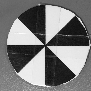
\includegraphics[width=3.5cm]{pythonpic/hubsan_region_around_detected_marker.png} 
\hfill 

\includegraphics[width=3.5cm]{pythonpic/hubsan_oriented_quality_template_oriented.png} 
\hfill 
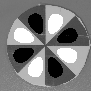
\includegraphics[width=3.5cm]{pythonpic/hubsan_merged_input_and_oriented_quality_template_oriented.png} 
\caption{Visualisation of how the quality of the detected marker in figure \ref{figHubsanInputImage} is assessed. 
A region centered above the detected marker is extracted, the quality template divides the extracted part 
of the image into three regions: expected white pixels, expected black pixels and don't care pixels. 
The template is rotated so it is aligned with the detected marker.} 
\label{figQualityEstimationProcess} 
\end{figure} 
 
% node end (ID_408776078)
% node start (ID_887206754)
% TEXT = Oriented marker
\subsection{The oriented marker} 
% node end (ID_887206754)
% node start (ID_810182894)
% TEXT = Removing a leg
Even though the plain marker contains some information about the orientation of the 
marker (as it is possible to discriminate between markers with different orientations), 
is is not possible for the pattern to point in a certain direction, for eg. specifying the orientation of a tracked object. 
By changing one of the black legs of the pattern to white, the pattern is given 
a unique orientation. 
This is illustrated in figure \ref{figMarkersWithOneMissingBlackElement}. 
 
% node end (ID_810182894)
% node start (ID_221364124)
% TEXT = figPlainMarkers
\begin{figure} 
\newcommand{\steplength}{30} 
\newcommand{\archlength}{1.6cm} 
\newcommand{\drawarch}[1]{\draw[color=black,fill=black] (2*#1:\archlength) arc(2*#1:2*#1+\steplength:\archlength) 
-- (0, 0) -- (2*#1:\archlength); } 
%\newcommand{\drawdot}{\draw[fill=black] (0, 0) circle (0.75mm);} 
\newcommand{\drawdot}{} 
\newcommand{\draworder}[1]{\draw (0, -2.2) node {n = #1};} 
\renewcommand{\archlength}{1cm} 
\begin{tikzpicture} 
\newcommand\order{2} 
\renewcommand\order{3} 
\begin{scope}[xshift=3.5cm] 
% Do calculation 
\pgfmathsetmacro{\steplength}{180 / \order}% 
\foreach \n in {0, \steplength, ..., 119}{\drawarch{\n}} 
\end{scope} 
\renewcommand\order{4} 
\begin{scope}[xshift=2*3.5cm] 
% Do calculation 
\pgfmathsetmacro{\steplength}{180 / \order}% 
\foreach \n in {0, \steplength, ..., 129}{\drawarch{\n}} 
\end{scope} 
\renewcommand\order{5} 
\begin{scope}[xshift=3*3.5cm] 
% Do calculation 
\pgfmathsetmacro{\steplength}{180 / \order}% 
\foreach \n in {0, \steplength, ..., 119}{\drawarch{\n}} 
\end{scope} 
\renewcommand\order{6} 
\begin{scope}[xshift=4*3.5cm] 
% Do calculation 
\pgfmathsetmacro{\steplength}{180 / \order}% 
\foreach \n in {0, \steplength, ..., 139}{\drawarch{\n}} 
\end{scope} 
\end{tikzpicture} 
\caption{Markers where one of the black legs have been removed to 
indicate an orientation of the marker. 
The markers have the orders ($n = 3 \ldots 6$).} 
\label{figMarkersWithOneMissingBlackElement} 
\end{figure} 
% node end (ID_221364124)
% node start (ID_1535548336)
% TEXT = Show modified quality template% node end (ID_1535548336)
% node start (ID_854015171)
% TEXT = Results
\section{Results} 
% node end (ID_854015171)
% node start (ID_129367257)
% TEXT = Required size for detecting a marker
\todo[inline]{Results on detecting markers with different sizes. Mention that markers can be detected reliably with $16 \times 16$ kernels, which is quite small.} 
 
\todo[inline]{Give results on the running time of the marker detector and how it scales with image and kernel size.} 
% node end (ID_129367257)
% node start (ID_1250748141)
% TEXT = Implementation is available at github
A python module implementing the algorithm is available on 
\url{https://github.com/henrikmidtiby/markerlocator}. 
% node end (ID_1250748141)
% node start (ID_1640560548)
% TEXT = Conclusion
\section{Conclusion} 
% node end (ID_1640560548)
% node start (ID_1395737850)
% TEXT = References
\printbibliography 
% node end (ID_1395737850)
% node start (ID_1361899356)
% TEXT = endofdocument
\end{document} 
% node end (ID_1361899356)
